% RESS major revision source.
\documentclass[final,number]{elsarticle}

\usepackage[T1]{fontenc}
\usepackage[utf8]{inputenc}
\usepackage{amsmath,amssymb}
\usepackage{booktabs}
\usepackage{array}
\usepackage{tabularx}
\usepackage{multirow}
\usepackage{graphicx}
\usepackage[hyphens]{url}
\usepackage{natbib}
\usepackage{algorithm}
\usepackage{algpseudocode}
\usepackage{threeparttable}
\usepackage{xcolor}
\setlength{\emergencystretch}{3em}
% The initial submission was read as containing spurious line-break hyphens
% (e.g. "com-puted", "counter-factual").  Automatic hyphenation is therefore
% disabled and overfull lines are absorbed by emergencystretch.
\hyphenpenalty=10000
\exhyphenpenalty=10000
\tolerance=3000
\graphicspath{{figures/}{./}}
\journal{Reliability Engineering \& System Safety}

\renewcommand{\topfraction}{0.9}
\renewcommand{\bottomfraction}{0.8}
\renewcommand{\textfraction}{0.07}
\renewcommand{\floatpagefraction}{0.8}

\begin{document}
\sloppy

\begin{frontmatter}

\title{From Explanation Agreement to Operability: A Restricted AC Screening Audit of GNN Explanations for Cascading-Failure Risk Assessment}

\author[aff1,aff2]{Zihao Huang\fnref{fn1}}
\author[aff1,aff2]{Yan Chen\corref{cor1}\fnref{fn2}}
\ead{cy@gxu.edu.cn}
\cortext[cor1]{Corresponding author}
\fntext[fn1]{ORCID: 0009-0006-5842-6516}
\fntext[fn2]{ORCID: 0000-0002-9950-684X}
\address[aff1]{Guangxi Key Laboratory of Digital Infrastructure, Guangxi Zhuang Autonomous Region Information Center, Nanning 530000, China}
\address[aff2]{School of Computer and Electronic Information, Guangxi University, Nanning 530000, China}

\begin{abstract}
Graph neural networks (GNNs) increasingly support cascading-failure risk assessment, and edge explanations are often read as candidate branches for corrective action. We show that the quantity most often used to validate such explanations, agreement with simulator cascade-path labels, is neither a measure of faithfulness to the classifier nor a measure of intervention operability. We separate three layers that are commonly conflated: edge-label agreement, model fidelity, and a restricted alternating-current (AC) screening test of a standardized top-$k$ branch-deletion counterfactual. The audit covers IEEE 24-bus, IEEE 39-bus, and UK systems; GNNExplainer, PGExplainer, GSAT, Grad-CAM, and SubgraphX; random, label-free, and shuffled-label controls; and a supervised edge-label predictor (SEP). Edge-label agreement is strongly confounded by branch-flow features: a label-free ranking by reactive-flow magnitude reaches 0.861 pooled edge balanced accuracy on IEEE 24, close to the SEP's 0.900, and classifiers trained on shuffled labels can reach similar values. Under a locked public-case AC screen that checks convergence, connectivity, and voltage, the SEP's raw top-5 deletions pass in 0.2\%, 2.5\%, and 64.0\% of accepted positive samples on IEEE 24, IEEE 39, and UK, respectively, whereas matched random deletions pass in 54.5\%, 7.7\%, and 100\%. On IEEE 24 a connectivity-preserving control shows that failures persist on connected networks through voltage violations, so they cannot be attributed to islanding alone; on IEEE 39 and UK the raw failures are primarily topological. Matched-sample, contingency-disjoint, intervention-budget, voltage-threshold, DC-versus-AC, and operating-point analyses bound the conclusions. A finite-budget wrapper can restore screening feasibility, but it rewrites part of the explanation and consumes a measurable number of AC solver calls. We conclude that restricted AC screening must be reported as a separate validation layer, and that edge-label agreement should not be described as faithfulness or operability.
\end{abstract}

\begin{keyword}
graph neural networks \sep explainable artificial intelligence \sep cascading failures \sep power-system reliability \sep AC power flow \sep topology intervention \sep explanation evaluation
\end{keyword}

\end{frontmatter}

\section{Introduction}\label{introduction}

Cascading failures are a defining reliability concern in interconnected power systems, and graph neural networks (GNNs) with post-hoc edge explanations are increasingly used to rank the branches that drive them~\citep{guo2023,cadini2017,gjorgiev2022,varbella2023gdl,varbella2024,liao2022}.

The mainstream recipe is now familiar. A GNN is trained on simulated cascade outcomes; an edge explainer---GNNExplainer, PGExplainer, SubgraphX, GSAT, or a gradient method---ranks branches for a graph; and the ranking is validated by its agreement with the simulator's cascade-path mask, usually reported as edge balanced accuracy (BACC), sometimes alongside fidelity and sparsity~\citep{varbella2024,ying2019,luo2020,yuan2021,miao2022,yuan2022}. \emph{The implicit assumption is that agreement with the simulator's cascade-path label validates the explanation.} If the highlighted branches coincide with the edges along which the simulated cascade propagated, the explanation is treated as faithful to the model and, frequently, as evidence that the highlighted branches are the ones worth acting on. Agreement then stops being one diagnostic among several and becomes the certificate that the explanation has recovered the mechanism the model uses---and, by extension, that removing those branches is a meaningful intervention.

That assumption has a crack, and it runs through both the explanation literature and the power-system literature. On the explanation side, agreement with a plausible reference is not the same as faithfulness to the model: plausibility and faithfulness are distinct properties, and a ranking can be plausible for reasons unrelated to the classifier's decision~\citep{jacovi2020,doshi2017,rudin2019}. Saliency maps can be largely insensitive to model parameters and still look convincing~\citep{adebayo2018}; fidelity benchmarks measure the effect of deleting or retaining features on the model output, not the physical consequence of acting on them~\citep{hooker2019,samek2017}; and taxonomic surveys of GNN explainers distinguish these criteria~\citep{yuan2022}, while broader XAI agendas identify the same evaluation gap across domains~\citep{longo2024}. Yet empirical studies often report the criteria side by side as if they were interchangeable. On the power-system side, a branch is not an actionable switch merely because it lies on a cascade path. Corrective topology actions are operating-point dependent and must satisfy AC power-flow constraints---convergence, connectivity, and voltage limits---after the switching~\citep{rolim1999,li2019,korad2013,li2017}. A cascade-path mask records where a simulated cascade travelled; it does not record whether removing that branch from a given operating state leaves a feasible network. A low physical screening pass rate is therefore not evidence that an explainer is poor; it is evidence that the selected branch set is not an operable switching action under the declared state. The two literatures therefore validate explanations with quantities that are, respectively, model-internal and simulation-internal, while the quantity that matters for action---post-switching AC feasibility---is not part of either validation vocabulary.

The crack is not hypothetical. In the audit reported here, a label-free ranking by reactive-flow magnitude reaches pooled edge BACC close to that of a supervised edge-label predictor (SEP) on IEEE 24 ($0.861$ versus $0.900$), and classifiers trained on shuffled labels can reach comparable values. Yet the SEP itself passes a restricted AC screen after top-5 deletion in only $0.2\%$ and $2.5\%$ of accepted samples on IEEE 24 and IEEE 39, while matched random deletions pass in $54.5\%$ and $7.7\%$. On IEEE 24, a connectivity-preserving control still fails through voltage violations and non-convergence, so the failures cannot be attributed to islanding alone. Agreement and operability can therefore move in opposite directions, and the direction depends on the system, the operating point, and the physical failure mechanism.

Why has this not been settled? Three barriers, not one. First, a \emph{methodological} barrier: explainers output edge rankings, not switching decisions. Turning a ranking into an auditable intervention requires re-solving the AC power flow after a topology change, checking convergence, islanding, and voltage limits, and separating the effect of the intervention from the operating point---none of which is part of standard explanation pipelines~\citep{ying2019,luo2020,yuan2021,miao2022}. Second, a \emph{data} barrier: cascade benchmarks such as PowerGraph provide graph labels and simulator-derived edge masks, but not intervention-feasibility labels, and the stored post-contingency branch flows are not a full dispatch from which an AC base case can simply be reloaded; reconstructing a feasible sample-conditioned state is itself a modelling problem~\citep{guo2023,varbella2024}. Third, an \emph{evaluation} barrier: fidelity, sparsity, and label agreement are cheap, model-internal, and benchmarkable, whereas AC screening is expensive, system-specific, and requires a declared protocol---which case, which contingency, which limits, which samples, and which controls. The field has optimized the metrics it can compute at scale, and those metrics do not contain the physical consequence. The evaluation barrier is also infrastructural: a credible audit needs a pinned AC solver, locked case files, exact branch mappings, and exact sample indices, none of which travel with a typical explanation benchmark.

This paper takes the evaluation barrier as its entry point. Rather than proposing another explainer, we treat an explanation as a \emph{counterfactual topology intervention} and ask what happens when its top-$k$ branches are removed from a declared operating case. The conceptual move is to separate three quantities that are commonly conflated---edge-label agreement, model fidelity, and restricted AC screening---and to evaluate them as separate layers rather than as interchangeable evidence. The primary protocol locks a reproducible public MATPOWER case and does not retain the initiating outage; a sample-conditioned protocol that reconstructs net injections and retains the outage is reported as a sensitivity analysis, not as the primary result. The audit covers three systems, five explanation methods and the supervised SEP, matched random controls, a label-free reactive-flow ranking, shuffled-label classifiers, a connectivity-preserving control, and a finite-budget wrapper. We report where the conclusions hold and where they do not: matched samples, contingency-disjoint splitting, intervention budget, voltage threshold, DC versus AC analysis, operating-point protocol, held-out scenarios, and a held-out backbone partition. The contribution is an audit framework and a set of empirical findings, not a new state-of-the-art explainer, an operational switching policy, or an estimate of long-run reliability.

The empirical analysis produces four findings. First, edge-label agreement is strongly confounded by branch-flow features. A label-free ranking by reactive-flow magnitude reaches pooled edge balanced accuracy close to that of a supervised edge-label predictor (SEP), and classifiers trained on shuffled labels reproduce much of the same agreement. The metric therefore cannot be read as faithfulness or as evidence that an explainer has recovered a causal cascade mechanism. Second, raw top-$k$ deletions frequently fail the restricted AC screen, and the failure is system-dependent: islanding is the largest single failure channel on IEEE 39 and UK, whereas IEEE 24 mixes islanding with voltage and non-convergence failures. Third, the failures are not merely an artefact of islanding. A connectivity-preserving control that removes only edges whose joint deletion leaves the bus graph connected still fails through voltage violations and non-convergence on IEEE 24 at essentially the raw rate, and it leaves residual AC failures on IEEE 39 and UK even though the pass rate improves substantially. Fourth, a finite-budget wrapper can restore screening feasibility, but it does so by rewriting part of the selected edge set and by consuming a measurable number of AC solver calls; wrapped output is therefore a modified intervention, not the original explanation.

These findings answer four research questions. \textbf{RQ1}: Does edge-label agreement predict the outcome of the restricted AC screen? \textbf{RQ2}: Which physical mechanisms cause screen failures, and how much of the failure survives when connectivity is preserved? \textbf{RQ3}: How sensitive are the conclusions to contingency-disjoint splitting, intervention budget, voltage threshold, DC versus AC analysis, and the operating-point protocol? \textbf{RQ4}: How should a finite-budget feasibility wrapper be reported so that its modification of the explanation and its computational cost remain auditable?

The contributions are threefold. First, we reframe an edge explanation as a counterfactual topology intervention and formalize a three-layer evaluation that separates edge-label agreement, model fidelity, and restricted AC screening; we show empirically that the first is not a proxy for the third. Second, we provide a protocol-separated comparison across three power systems, five random seeds where resources permit, multiple explainer families, matched random controls, label-free and shuffled-label controls, and a connectivity-preserving control that isolates AC-constrained failures from disconnection. Third, we quantify the boundaries introduced by matched samples, contingency-disjoint splitting, intervention budget, voltage threshold, DC power flow, operating-point reconstruction, and feasibility repair.

The remainder of the paper is organized as follows. Section~\ref{related_work} reviews cascading-failure reliability, graph learning, explanation methods, and physics-aware evaluation. Section~\ref{problem_formulation_and_audit_protocol} defines the three layers, the operating states, the restricted AC screen, the wrapper, and the statistical protocol. Section~\ref{experimental_design} describes the systems, data, backbones, explainers, sample selection, and reproducibility package. Section~\ref{results} reports the results. Section~\ref{discussion} discusses implications and limitations, and Section~\ref{conclusions} concludes.

\section{Related work}\label{related_work}

\subsection{Cascading-failure reliability and topology actions}\label{cascading_failure_reliability_and_topology_actions}

Power-system cascading failures emerge from coupled topological and electrical mechanisms. Classical reliability and security assessment uses contingency analysis, AC or DC power flow, dynamic simulation, and probabilistic models to evaluate whether the system remains within acceptable limits after disturbances~\citep{guo2023,cadini2017,gjorgiev2022,zhang2022cyber,zhu2023,gao2025}. Global sensitivity and uncertainty-quantification methods are often used to prioritize the reliability and risk drivers underlying such assessments~\citep{rahman2011,zhang2014,yao2023}, and adaptive network reliability methods model how component degradation propagates through the grid~\citep{dehghani2021}. Transmission switching has also been investigated as a corrective or preventive action, with early and recent formulations emphasizing that candidate switching decisions must remain feasible under the relevant network constraints~\citep{rolim1999,li2019,korad2013,li2017,ding2016,zhang2024rl}. Our study does not optimize a corrective action. Instead, it uses topology deletion as a standardized counterfactual stress test for an explanation and reports the physical mechanism by which the resulting state fails a declared screen.

\subsection{Graph learning for power systems}\label{graph_learning_for_power_systems}

GNNs have been applied to power flow, optimal power flow, contingency screening, and security assessment because message passing can represent interactions along network branches~\citep{liao2022,su2023,ngo2024}. PowerGraph provides simulated graph-level cascading-failure tasks with bus features, branch features, graph labels, and edge masks derived from the simulated cascade path~\citep{varbella2024,varbella2023}. Geometric deep learning has also been tailored to online cascade prediction~\citep{varbella2023gdl}; graph models have been proposed for power-grid fault detection~\citep{bosso2025} and fault localization~\citep{gjorgiev2023}, with varying interpretability claims. We use these masks as evaluation labels, not as prescriptive switching labels. This distinction is central: the edge that participated in a cascade is not necessarily an edge that should be opened in a corrective action.

\subsection{Graph explanation methods}\label{graph_explanation_methods}

Post-hoc graph explanation methods assign importance to graph components after a predictor has been trained. GNNExplainer optimizes a compact mask that preserves a target prediction~\citep{ying2019}. PGExplainer amortizes explanation generation through a parameterized network~\citep{luo2020}. SubgraphX uses Monte Carlo tree search and Shapley-value approximations to identify explanatory subgraphs~\citep{yuan2021}. Gradient and Grad-CAM-style methods use local derivatives, while GSAT jointly learns stochastic attention intended to improve interpretability and generalization~\citep{miao2022}. These methods represent optimization-based, learned, search-based, and gradient-based explanation families. Their objectives do not enforce AC feasibility after topology changes. The broader post-hoc-explainability literature has also questioned whether post-hoc explanations are sufficient for high-stakes downstream decisions~\citep{longo2024,rudin2019}, and explainable-AI methods have been applied to reliability-relevant fault diagnostics in transmission assets~\citep{hsu2025}.

\subsection{Evaluating explanations: fidelity, agreement, and physical consequence}\label{physics_aware_explanation_evaluation}

Explanation evaluation is commonly separated into fidelity, sparsity, stability, and agreement with a reference label. Fidelity-based tests delete or retain the explained features and measure the change in the model output~\citep{samek2017,hooker2019}. Sanity checks show that some saliency maps are largely insensitive to model parameters and can therefore appear faithful without reflecting the model~\citep{adebayo2018}. These tests probe the model--explainer relationship, not the physical consequence of acting on the explanation. Physics-informed learning often introduces conservation laws, simulator losses, or feasibility constraints during training~\citep{misyris2020,xu2023,zhou2023pin,mei2024,li2026,he2025}. These physics-guided neural models have been deployed for reliability assessment of multi-state systems and power assets, but their objective remains prediction or reliability estimation rather than auditing the consequence of a discrete topology action. Our audit closes this evaluation gap by applying the explained top-$k$ edge set to a fixed operating case and classifying the resulting AC outcome. It does not reinterpret the explanation label as an operational recommendation, and it does not claim that the audit is a faithfulness test.

\section{Problem formulation and audit protocol}\label{problem_formulation_and_audit_protocol}

\subsection{Graph prediction and edge explanations}\label{graph_prediction_and_edge_explanation}

Let a power-system state be represented by a graph $G=(V,E,X,A)$, where $V$ and $E$ are buses and branches, $X$ contains node features, and $A$ contains edge features. The binary graph classifier $f_\theta(G)$ estimates whether the simulated disturbance leads to non-zero demand not served. An explainer produces one score $s_e \in \mathbb{R}$ for each currently available physical edge. For a budget $k$, the standardized intervention is the set
\begin{equation}
S_k = \operatorname{TopK}_{e\in E}(s_e,k).
\label{eq:topk}
\end{equation}
The experiment removes the branches in $S_k$ from a declared operating case and evaluates the modified network. This operation is deliberately simple and common to all methods. It is a counterfactual stress test, not an optimized switching action.

\subsection{Three layers and what each quantity measures}\label{three_layer_evaluation}

The workflow is summarized in Figure~\ref{fig:workflow}, and Table~\ref{tab:layers} summarizes the three layers and the quantities reported in each. The first layer measures \emph{edge-label agreement}. Simulator-derived cascade-path masks in \texttt{exp.mat} define the positive edge labels. For a ranking that selects a set $S$ of edges, we report pooled edge balanced accuracy
\begin{equation}
A_{\mathrm{edge}}=\frac{1}{2}\left(\frac{\mathrm{TP}}{\mathrm{TP}+\mathrm{FN}}+\frac{\mathrm{TN}}{\mathrm{TN}+\mathrm{FP}}\right),
\label{eq:bacc}
\end{equation}
where TP, FP, TN, and FN are summed over all evaluated graphs and all available branches. Pooling avoids the single-class artefact that arises when a graph contains no cascade-path edge: a per-graph balanced accuracy is undefined in that case, and common implementations return a value that depends on the prediction rather than on discrimination. We use the same definition for the graph-level classifier, with graphs rather than edges as the units, and denote it $A_{\mathrm{graph}}$. The chance level of $A_{\mathrm{edge}}$ is not necessarily $0.5$ when the label distribution is highly concentrated on a feature subspace; Section~\ref{edge_label_agreement_is_not_faithfulness} reports an explicit permutation null.

The first layer also includes \emph{model fidelity}. For an explanation set $S$ we define
\begin{equation}
\mathrm{Fid}^{+}=\Pr\left[f_\theta(G_{S})=f_\theta(G)\right],\qquad
\mathrm{Fid}^{-}=\Pr\left[f_\theta(G_{\setminus S})\neq f_\theta(G)\right],
\label{eq:fidelity}
\end{equation}
where $G_S$ retains only the explained edges and $G_{\setminus S}$ removes them. $\mathrm{Fid}^{+}$ measures whether the explanation is sufficient to preserve the prediction, and $\mathrm{Fid}^{-}$ measures whether deleting the explanation flips it. These are model-centric quantities and do not involve the power-flow screen.

The second layer measures physical operability as a \emph{restricted AC screening pass rate}. For sample $i$ in the accepted positive-class evaluation subset $\mathcal{S}^{+}$, let $F_i(S_k)=1$ when the AC screen converges and satisfies the declared voltage and connectivity checks after the edges in $S_k$ are removed. The conditional screening pass rate is
\begin{equation}
\mathrm{PFR@}k = \frac{1}{|\mathcal{S}^{+}|}\sum_{i\in\mathcal{S}^{+}}\mathbb{1}[F_i(S_k)=1].
\label{eq:pfr}
\end{equation}
We retain the acronym PFR for continuity with the initial submission, but throughout this revision it denotes a \emph{restricted AC screening pass rate}, not comprehensive AC operability. For the primary public-case screen, $F_i$ is a predicate over convergence, connectivity, and voltage only; thermal loading is recorded as a separate taxonomy channel and is not a rejection condition (Section~\ref{restricted_ac_screen}). Infeasible screening outcomes are classified as island, non-converged, or voltage violation. Reporting the taxonomy is necessary because equal PFR values can arise from different reliability mechanisms. A screening failure is not, by itself, proof that the physical system is inoperable: non-convergence in particular is a solver outcome, and we treat it as a failure to pass the declared screen rather than as demonstrated infeasibility. Equally, a failed screen does not establish poor explanation quality: it shows that the selected set is not an operable intervention under the declared protocol, not that the explainer failed to identify a diagnostically important branch.

We also report a severity-weighted screening risk,
\begin{equation}
R_{\mathrm{sev}}=\frac{1}{|\mathcal{S}^{+}|}\sum_{i\in\mathcal{S}^{+}} r_i,\qquad
r_i=\begin{cases}0,&F_i(S_k)=1,\\
\min\!\bigl(1,\;\epsilon_i/0.25\bigr),&\text{voltage violation,}\\
1,&\text{island or non-converged,}\end{cases}
\label{eq:risk}
\end{equation}
where $\epsilon_i$ is the larger of the maximum under-voltage and over-voltage violation magnitudes in p.u.\ relative to the screening interval. The penalty scale $0.25$ p.u.\ equals the width of the declared voltage interval $[0.85, 1.10]$ p.u., so the voltage term saturates when the worst violation reaches the full interval width; this scale is a declared convention of the audit rather than a utility-specific damage curve. $R_{\mathrm{sev}}$ therefore rises smoothly with voltage stress and saturates at hard failures, without conflating distinct failure mechanisms into a single count. It is a supplementary diagnostic, not a primary endpoint. It is computed only for the rankings whose per-instance artefacts record the voltage and connectivity detail required by Eq.~\eqref{eq:risk}; in the present archive this is GNNExplainer, the matched random control, and the truth anchor. We report these values in Section~\ref{raw_interventions_fail_through_different_physical_mechanisms} and do not impute them for other methods. It is not a demand-not-served measure and is reported as action-driven screening severity. The field named \texttt{mean\_risk} in the archived artefacts is the same quantity as $R_{\mathrm{sev}}$; the manuscript uses only $R_{\mathrm{sev}}$ to avoid a second notation.

The third layer measures computational and intervention burden, including wall-clock time, intervention size (number of branches switched out), candidate replacements introduced by a wrapper, and, where available, AC solver calls. These measurements characterize the audit workload rather than a universal method-speed ranking or an economic switching cost.

\begin{table*}[!htb]
\centering
\caption{The three evaluation layers and the quantities reported in each. Layer 1 is split into prediction (1a), edge-label agreement (1b), and model fidelity (1c). The layers answer different questions and are not interchangeable. $A_{\mathrm{edge}}$ is agreement with a simulator mask, not faithfulness; PFR is a restricted AC screening pass rate, not comprehensive AC operability or long-run reliability.}
\label{tab:layers}
\begingroup\hyphenpenalty=100\exhyphenpenalty=100\tolerance=2000
\scriptsize
\setlength{\tabcolsep}{3pt}
\begin{tabularx}{\textwidth}{@{}l>{\raggedright\arraybackslash\hsize=0.9\hsize}X>{\raggedright\arraybackslash\hsize=1.5\hsize}X>{\raggedright\arraybackslash\hsize=0.9\hsize}X>{\raggedright\arraybackslash\hsize=0.7\hsize}X@{}}
\toprule
Layer & Quantity & Definition & Supports & Does not support \\
\midrule
1a. Prediction & $A_{\mathrm{graph}}$ & Graph-level balanced accuracy of $f_\theta$ & Predictive performance on the declared split & Explanation quality or transfer \\
1b. Edge-label agreement & $A_{\mathrm{edge}}$ (Eq.~\ref{eq:bacc}) & Pooled edge BACC against simulator cascade-path masks & Agreement with the benchmark label & Faithfulness, causal recovery, or operability \\
1c. Model fidelity & $\mathrm{Fid}^{+}$, $\mathrm{Fid}^{-}$ (Eq.~\ref{eq:fidelity}) & Prediction change after retaining/removing explained edges & Whether the explanation drives the classifier & Physical \mbox{consequence} or label correctness \\
2. Physical screening & $\mathrm{PFR@}k$ (Eq.~\ref{eq:pfr}) & Pass rate of convergence, connectivity, and voltage checks after top-$k$ deletion & A declared counterfactual screen & Comprehensive AC operability, reliability, or switching policy \\
3. Burden & Time, replacements, AC calls & Measured or bounded cost of producing the intervention & Auditable cost accounting & Economic switching cost or universal speed ranking \\
\bottomrule
\end{tabularx}
\endgroup
\end{table*}

\begin{figure}[!htb]
\centering
\makebox[\textwidth][c]{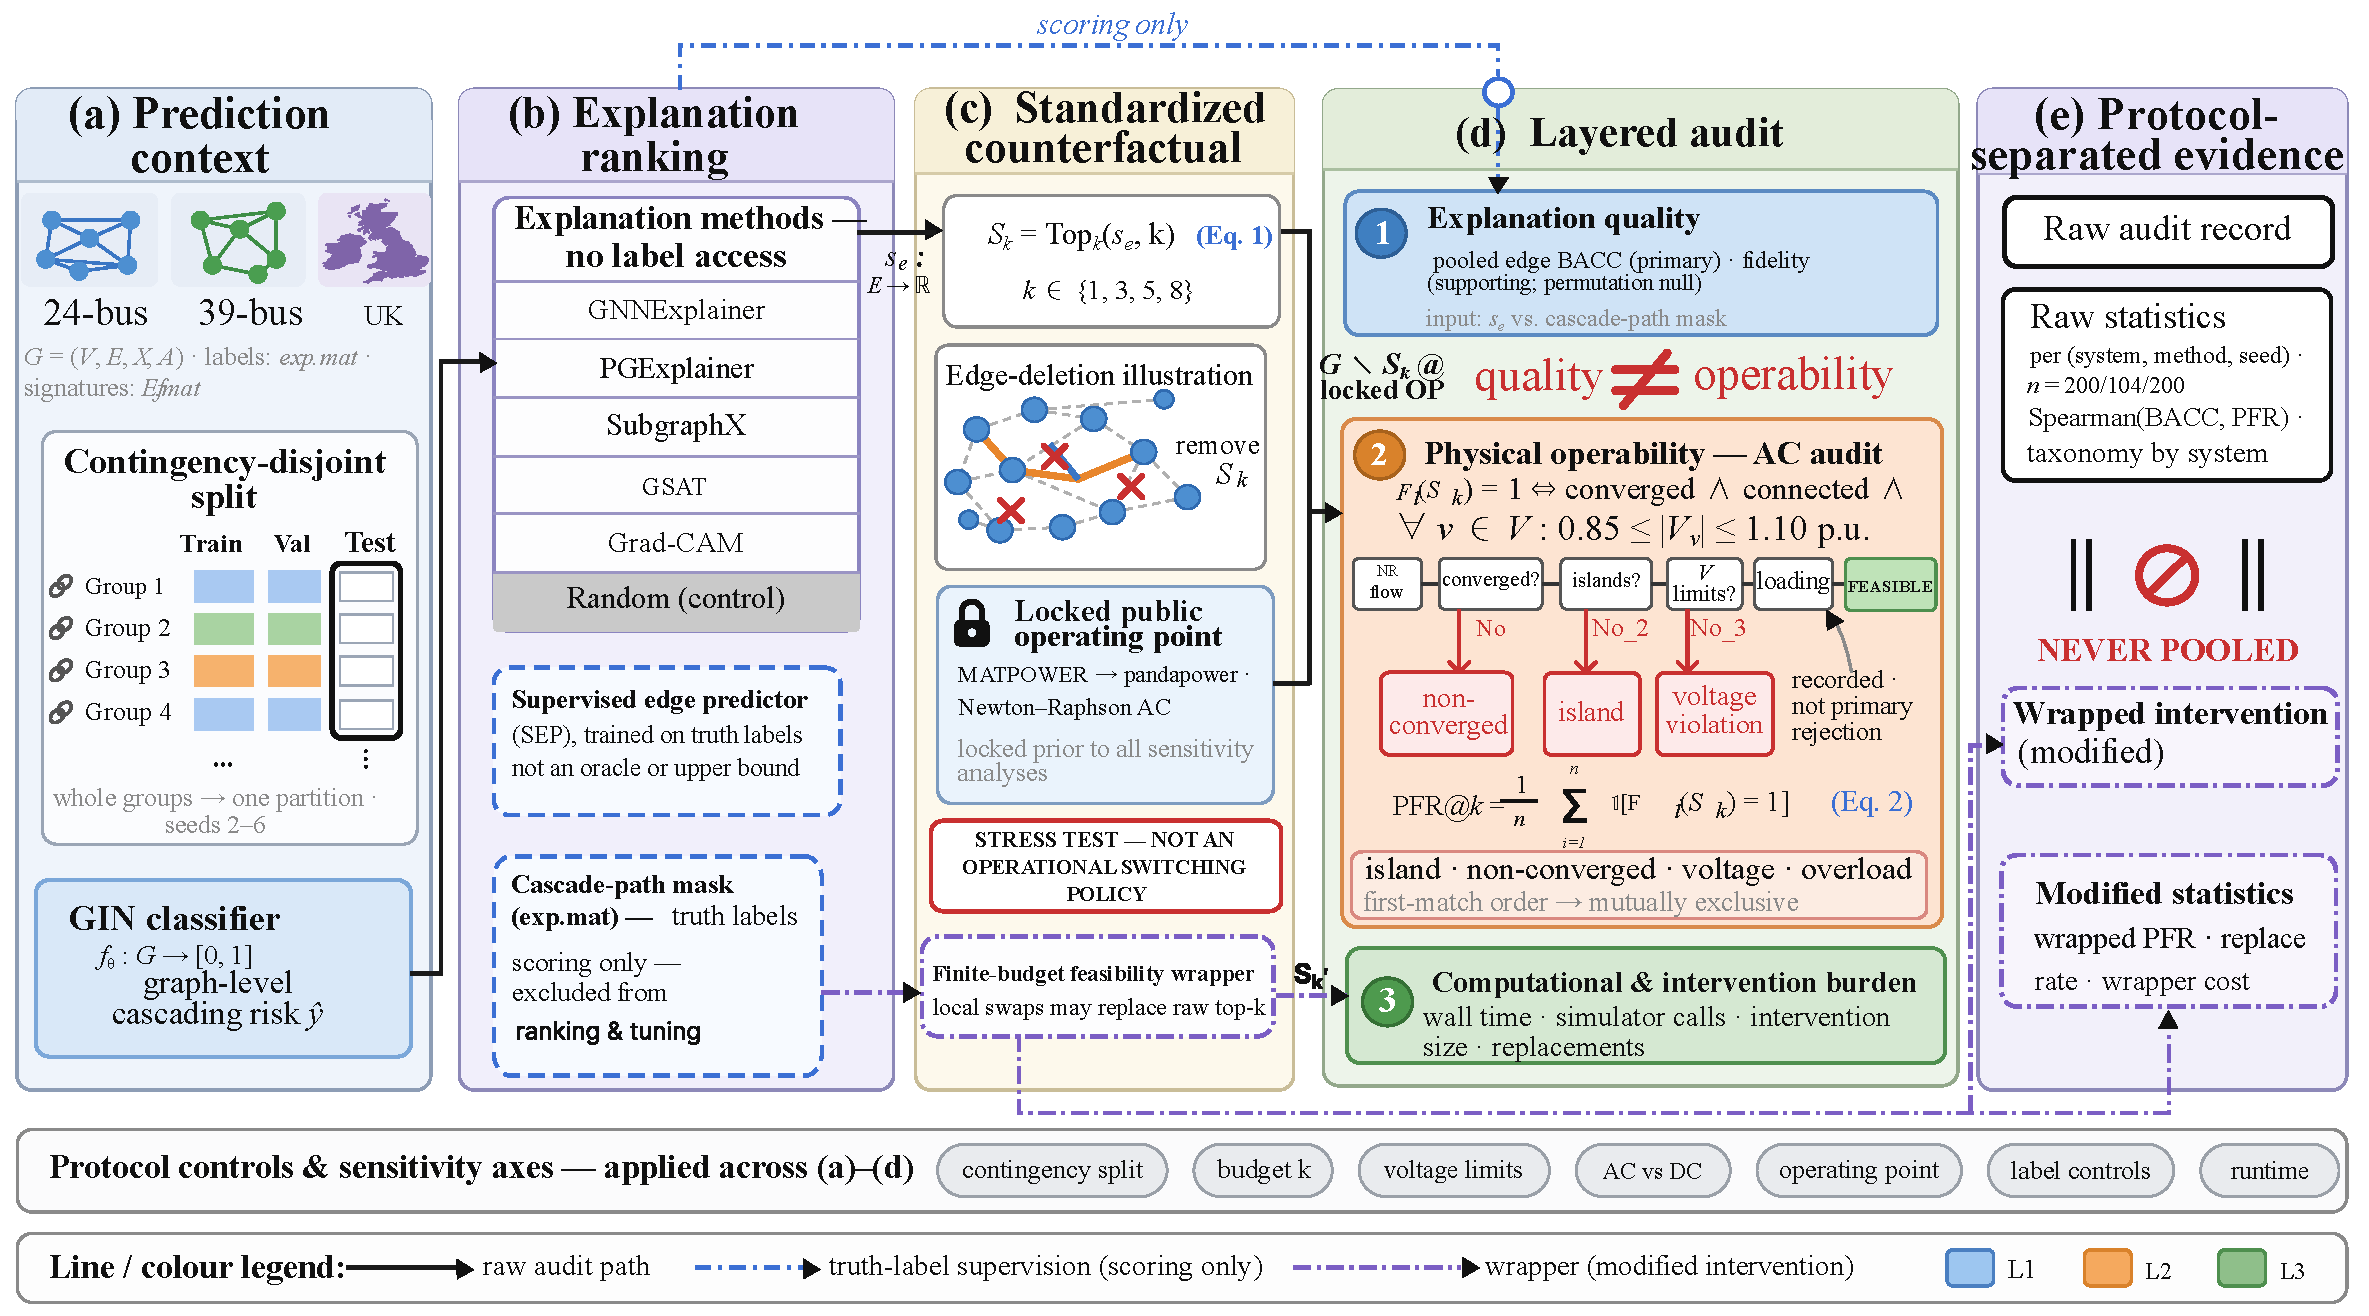
\includegraphics[width=1.35\textwidth]{figures/figure_1_workflow.pdf}}
\caption{Reliability-oriented audit workflow. (a) Prediction context: graphs from the IEEE 24-bus, IEEE 39-bus, and UK systems feed a common GIN classifier; the contingency-disjoint split used for the scenario-transfer test is illustrated (the main backbone uses a random 85/5/10 split). (b) Five explanation methods and a random control rank branch importance without label access; the supervised edge-label predictor (SEP) is trained on truth edge labels in the training split but is not an oracle or an upper bound. (c) The raw top-$k$ set $S_k$ is applied as a standardized deletion counterfactual to a locked public operating point under Newton--Raphson AC power flow. (d) Explanation quality (pooled edge BACC with a permutation null, and model fidelity), physical operability with a four-outcome, mutually exclusive taxonomy (feasible, island, non-convergence, or voltage violation; thermal overload is recorded but excluded from the rejection criterion), and computational/intervention burden are audited as separate layers. (e) Raw and wrapper-modified evidence are never pooled; wrapped PFR, replacement rate, and wrapper cost are reported separately. Evaluation is held out at the sample level (matched slices, 20--49 purge gap), the scenario level (contingency-disjoint groups), and, for six methods, the backbone level (the GIN test partition). Top-$k$ deletion is a counterfactual stress test, not an operational switching policy.}
\label{fig:workflow}
\end{figure}

\subsection{Operating states at each stage}\label{operating_states}

The interpretation of any screening rate depends on the topology and operating state used at each stage. Table~\ref{tab:states} states these choices explicitly; this resolves an ambiguity in the initial submission, where the methods described a fixed public MATPOWER operating point while the experiments described a sample-conditioned reconstruction.

The prediction and explanation stages use the PowerGraph sample graph. Its topology is the original network with the initiating-outage branches removed, where the initiating outage is operationalized as the set of branches whose four post-contingency features are exactly zero. The node features are the three benchmark bus features, and the branch features are the post-contingency active flow, reactive flow, reactance, and rating. The graph label is binary demand-not-served. Explanations are generated only for the currently available branches; the removed outage branches are not candidates.

The primary physical audit uses the locked public MATPOWER case. The full public topology is restored, the public dispatch is retained, and the initiating outage is \emph{not} retained. The top-$k$ explanation branches are switched out of this public case, and the AC screen is evaluated. This protocol answers: if the branches highlighted in a post-cascade explanation were opened from the public base case, would the resulting state pass the declared screen? It does not claim to reconstruct the state after the simulated cascade.

The sample-conditioned sensitivity protocol is different and is reported separately. It reconstructs net injections from the stored post-contingency branch-flow matrix $E_f$, retains the sample's initiating-outage branches as out of service, and then removes the same top-$k$ branches. Its empty-set control is the reconstructed base state. This protocol is closer to the sample's electrical state but depends on a reconstruction whose base state is not always feasible. It is therefore a sensitivity analysis, not the primary protocol. Both protocols are evaluated on the same samples and, in the operating-point comparison of Section~\ref{operability_is_sensitive}, on the \emph{same raw top-$k$ sets}; no feasibility-guided selection is applied there.

\begin{table*}[!htbp]
\centering
\caption{Topology and operating state at each stage of the audit. The primary public-case audit does not retain the initiating outage; the sample-conditioned sensitivity does.}
\label{tab:states}
\begingroup\hyphenpenalty=100\exhyphenpenalty=100\tolerance=2000
\scriptsize
\setlength{\tabcolsep}{3pt}
\begin{tabularx}{\textwidth}{@{}l>{\raggedright\arraybackslash\hsize=1.1\hsize}X>{\raggedright\arraybackslash\hsize=0.9\hsize}X>{\raggedright\arraybackslash\hsize=0.9\hsize}X>{\raggedright\arraybackslash\hsize=1.1\hsize}X@{}}
\toprule
Stage & Topology & Injections / dispatch & Initiating outage & Purpose \\
\midrule
Prediction & Sample graph: outage branches removed; available branches only & Benchmark bus features; post-contingency branch features & Removed from graph & Graph label $f_\theta(G)$ \\
Explanation & Same sample graph & Same features & Not a candidate & Rank available branches \\
Contingency signature & Zero-flow branch set in $E_f$ & Not used & Defines the group & Contingency-disjoint split \\
Public-case screen (primary) & Full public MATPOWER case & Public case dispatch & \emph{Not retained} & Standardized counterfactual screen \\
Sample-conditioned screen (sensitivity) & Public case minus outage branches and minus $S_k$ & Reconstructed from $E_f$ & \emph{Retained} & State-conditional sensitivity \\
Wrapper & Public case minus the repaired set & Public case dispatch & Not retained & Finite-budget feasibility repair \\
\bottomrule
\end{tabularx}
\endgroup
\end{table*}

\subsection{Restricted AC screening criterion}\label{restricted_ac_screen}

The screen is a convergence--connectivity--voltage check, not a full AC security assessment. Table~\ref{tab:solver} lists the settings. We use pandapower 3.5.4~\citep{thurner2018} with the Newton--Raphson solver, automatic initialization (DC power flow when available, flat start otherwise), a mismatch tolerance of $10^{-8}$ MVA, and \texttt{max\_iteration='auto'}, which pandapower 3.5.4 resolves to 10 Newton--Raphson iterations. Generator reactive limits are not enforced, generator active-power limits are likewise not enforced, and no redispatch is performed; PV buses hold their voltage setpoint and the slack bus balances the residual. The original case's transformer taps, shunts, and voltage setpoints are retained. Loads are constant-power, as created by the MATPOWER converter.

The screening voltage interval is $[0.85,1.10]$ p.u. for the primary analysis. Stricter lower limits of 0.90 and 0.95 p.u.\ are evaluated as sensitivity analyses (Section~\ref{operability_is_sensitive}). For the primary public-case screen, connectivity is checked by pandapower's connectivity preprocessing and by the presence of undefined bus voltages; a converged run with any undefined bus voltage is classified as an island. Non-convergence is recorded when the solver raises an exception or reports that it did not converge and takes precedence over the island label, so the taxonomy remains mutually exclusive. Thermal loading is computed but not used as a rejection condition because the source public cases contain design-specific baseline overloads; it is recorded as a separate channel with a threshold of $10^{9}$\% in the primary screen. This is why the consolidated table contains no overload rejection column.

Branch mapping is explicit. The benchmark's \texttt{blist.mat} provides one row per physical branch as a pair of bus numbers. Each row is matched to a pandapower line, transformer, or impedance element by its endpoint pair; parallel branches are assigned one-to-one in the order in which they appear, so no element is used twice. The IEEE 24-bus case maps to 33 lines and 5 transformers; the IEEE 39-bus case to 35 lines and 11 transformers; the UK case to 86 lines, 4 transformers, and 9 impedance elements. All 183 benchmark branches map with zero unmatched rows. Cross-voltage-level branches with zero tap ratio are represented as impedance elements by the converter and are switched out through the same mapping. The mapping tables and a verification script are included in the reproducibility package.

\begin{table*}[!htbp]
\centering
\caption{Restricted AC screening criterion and solver settings for the primary public-case screen. The screen is a convergence--connectivity--voltage check; it is not a comprehensive AC security assessment.}
\label{tab:solver}
\begingroup\hyphenpenalty=100\exhyphenpenalty=100\tolerance=2000
\scriptsize
\setlength{\tabcolsep}{3pt}
\begin{tabularx}{\textwidth}{@{}l>{\raggedright\arraybackslash\hsize=1.1\hsize}X>{\raggedright\arraybackslash\hsize=0.9\hsize}X@{}}
\toprule
Item & Setting & Consequence for interpretation \\
\midrule
Engine & pandapower 3.5.4, Newton--Raphson, \texttt{numba=False} & Deterministic per-run solver; platform differences can affect borderline cases \\
Initialization & \texttt{init='auto'} (DC initialization when available, flat start otherwise) & Not a warm start from the sample state \\
Tolerance / iterations & $10^{-8}$ MVA; \texttt{max\_iteration='auto'} (10 Newton--Raphson iterations in pandapower 3.5.4) & Convergence failure is a solver outcome, not proof of infeasibility \\
Reactive limits & \texttt{enforce\_q\_lims=False} & Generator reactive limits are not enforced \\
Active-power limits & Not enforced; no redispatch & Dispatch is not re-optimised; the slack absorbs the residual \\
Slack & Original case slack bus; PV generators hold voltage setpoint & Residual active-power mismatch is absorbed by the slack \\
Voltage limits & $[0.85,1.10]$ p.u.; 0.90 and 0.95 sensitivity & Declared N-1-style interval, not a utility-specific limit \\
Connectivity & Pandapower connectivity preprocessing; undefined bus voltage = island & Islanding is separated from voltage and convergence failures \\
Thermal loading & Recorded; threshold $10^{9}$\% (not a rejection condition) & Baseline case overloads do not drive the screen \\
Branch mapping & Endpoint matching from \texttt{blist.mat}; one-to-one for parallel branches & 183/183 branches mapped; transformers and impedances included \\
Non-convergence & Exception or \texttt{converged=False} & Classified as screen failure, not as demonstrated physical infeasibility \\
\bottomrule
\end{tabularx}
\endgroup
\end{table*}

\subsection{Public-case and sample-conditioned protocols}\label{public_case_counterfactual_feasibility_audit}

The primary protocol is tied to a reproducible public operating point. It loads the public MATPOWER System.m case for each network and converts it to a pandapower representation. The candidate branches are switched out while the public operating point is retained, and the AC screen is then executed. The public case was locked before the sensitivity analyses because it is directly reproducible and has a feasible base state.

Two caveats follow directly from this design and are retained throughout the manuscript. First, the audited samples are the accepted positive-class cascade evaluation graphs (Section~\ref{sample_selection}), so every PFR reported here is conditional on those samples; it is not a rate over the overall risk population and is therefore not an estimate of long-run system reliability. Second, because the retained operating point is from the public case, a passing result indicates only that the public-case topology-after-deletion is solvable within the declared constraints; it does not assert that the deletion would be feasible at the sample-specific dispatch.

The sample-conditioned alternative reconstructs net injections from the simulated branch-flow matrix and applies the sample's initial contingency. Net injections are obtained by summing the stored post-contingency branch flows at each bus. Positive net injections become PV generators with fixed active power and unconstrained reactive limits; negative injections become constant-power loads; the bus with the smallest absolute net injection is used as the slack. The initiating-outage branches are out of service; the same convergence, connectivity/island, and voltage criteria are applied as in the primary public-case screen. This protocol is reported only as a sensitivity analysis. Its base state is not always feasible (97.0\%, 88.5\%, and 100.0\% on IEEE 24, IEEE 39, and UK, respectively), so its rates and its failure taxonomy are reported separately from the public-case results. Section~\ref{operability_is_sensitive} reports both protocols on identical raw top-$k$ sets and reports the reconstructed base rate separately.

\subsection{Contingency-disjoint splitting}\label{contingency_disjoint_splitting}

Random graph splits can place different operating points associated with the same initiating contingency into both training and test partitions. To test this dependence, we define a contingency signature from the set of physical edges whose four branch features are zero in $E_f$. Samples with the same signature are assigned wholly to train, validation, or test. A greedy group allocation balances graph count and positive-class count without splitting a contingency group. Five seeds (2--6) are used for the GIN backbone. This signature is a conservative grouping variable: a branch with exactly zero flow after the cascade may be out of service for reasons other than the initiating outage, so the signature can merge contingencies that are not physically identical. The split is therefore a stress test of scenario dependence, not a verified outage reconstruction.

\subsection{Finite-budget wrapper}\label{feasibility_wrapper}

The wrapper scans a finite candidate ordering and searches for exactly $k$ edges whose joint deletion passes the AC screen. Algorithm~\ref{alg:wrapper} gives the procedure. It first greedily accepts the next-ranked edge only if the partial set passes the screen. If the greedy set reaches $k$ edges, the local-swap phase considers one-edge replacements drawn from the first $P$ ranked edges (default $P=8$) and accepts a replacement only if the new set passes the screen and increases the sum of explainer scores. If the greedy phase cannot reach $k$ edges, the set is returned as incomplete and counted as a screen failure. The wrapper therefore has two distinct costs: the greedy phase can audit up to the number of available branches, and the local-swap phase can audit up to $kP$ replacements. The widely quoted $kP=40$ bound covers only the local-swap phase and excludes the greedy audits; Section~\ref{wrapper_changes_explanation} reports the measured distribution instead of treating 40 as a hard cap.

\begin{algorithm}[t]
\caption{Local-swap screening wrapper}\label{alg:wrapper}
\begin{algorithmic}[1]
\Require ranking $\pi$ of available branches, scores $s$, budget $k$, pool size $P$
\State $C\gets\emptyset$
\For{$e\in\pi$ in descending score order}
  \If{$|C|=k$} \textbf{break} \EndIf
  \If{$\mathrm{screen}(C\cup\{e\})$ passes} $C\gets C\cup\{e\}$ \EndIf
\EndFor
\If{$|C|<k$} \Return incomplete \EndIf
\State $B\gets C$; \quad $b\gets\sum_{e\in C}s_e$
\For{$e_{\mathrm{old}}\in C$}
  \For{$e_{\mathrm{new}}\in\pi[1{:}P]$, $e_{\mathrm{new}}\notin C$}
    \State $C'\gets C\setminus\{e_{\mathrm{old}}\}\cup\{e_{\mathrm{new}}\}$
    \If{$\mathrm{screen}(C')$ passes and $\sum_{e\in C'}s_e>b$}
      $B\gets C'$; \quad $b\gets\sum_{e\in C'}s_e$
    \EndIf
  \EndFor
\EndFor
\State \Return $B$
\end{algorithmic}
\end{algorithm}

\subsection{Statistical analysis and matched samples}\label{statistical_analysis}

Five-seed estimates are summarized by mean and sample standard deviation. For the contingency-disjoint backbone experiment we report a two-sided 95\% interval based on the $t$ distribution with four degrees of freedom, and we state explicitly that this interval describes variation across the five observed training seeds, not sampling uncertainty over graphs or contingencies. The accepted samples overlap across seeds, so the interval is not a population confidence interval. For the binary screening outcomes we report a non-parametric cluster bootstrap that resamples seed identities and recomputes the pooled rate (2000 replicates); this preserves the between-seed dependence but still does not account for overlap among the accepted graphs.

Table~\ref{tab:outcomes} reports, for each method and system, the pooled PFR, its cluster-bootstrap interval, the mean difference from the method's own matched random control, a paired seed-level effect size, and the corresponding bootstrap interval. The matched random control is generated on the same sample and from the same candidate-edge set as the method, so the difference is not confounded by different denominators. A Wilcoxon signed-rank test on the per-seed differences is reported in the archive as \texttt{ress\_statistical\_revision.json} under \texttt{data/results\_revision/results\_statistics}; with five seeds the minimum attainable two-sided $p$-value at five non-zero pairs is $0.0625$, so we do not treat significance thresholds as decisive.

The edge-label agreement analysis uses the pooled definition in Eq.~\eqref{eq:bacc}. We report the observed value and an explicit permutation null obtained by retraining the same logistic scorer on shuffled training labels with the same split and the same features; the null distribution is therefore specific to the feature set and label prevalence rather than assuming a chance level of 0.5. For each system we use ten permutations per seed (50 models per system) and report the mean, range, and the fraction of permutations that reach or exceed the observed agreement. This is a diagnostic of the metric, not a hypothesis test about explainer quality.

Finally, we distinguish the population to which each interval applies. The cluster-bootstrap interval describes the five observed seed identities. The permutation null describes the variability of the agreement statistic under label shuffling for the fixed accepted sample. Neither describes future contingencies, other networks, or the full risk population. We therefore report them as descriptive uncertainty summaries and avoid population-level language.

Every explanation method except the SEP is label-free at ranking time, and all but GSAT are post-hoc. The SEP is an explicit exception: it learns from truth-edge labels in the training split and is called a supervised edge-label predictor, not an oracle and not an upper bound on explanation quality. The label-free reactive-flow ranking and the shuffled-label classifiers are controls, not deployable explainers.

\section{Experimental design}\label{experimental_design}

\subsection{Systems and data}\label{systems_and_data}

We use the IEEE 24-bus, IEEE 39-bus, and UK systems from the PowerGraph cascading-failure benchmark~\citep{varbella2024,varbella2023}. The stored simulation sets contain 21{,}500, 28{,}000, and 64{,}000 graphs, respectively. Positive-class cascade graphs number 4334 (20.2\%), 2509 (9.0\%), and 2236 (3.5\%). Explainable positive graphs, defined as positive graphs with a non-null cascade-path mask, number 3416 (15.9\% of all graphs), 154 (0.55\%), and 2236 (3.5\%). The IEEE 39-bus explainable-positive population is therefore small: the n=104 evaluation slice covers a large fraction of the 154 available graphs, and the five seeds draw partially overlapping subsets. This limits the interpretable scope of the IEEE 39-bus rates and is stated wherever those rates are used.

Each graph contains three bus features and four branch features: active power flow, reactive power flow, line reactance, and line rating. Binary labels indicate whether demand not served is non-zero after the simulated cascade. Explanation masks identify the physical branches involved in the simulated cascade. The IEEE 118-bus data are not included in the cross-system main analysis because the number of valid positive explanation samples was insufficient under the locked filtering protocol; the archived IEEE 118-bus runs are retained in the data package for completeness but are not used for any claim in this paper.

The benchmark's branch list provides one row per physical branch. The public case files are the MATPOWER System.m cases distributed with PowerGraph. The number of branches per system and their mapping to pandapower elements are reported in Table~\ref{tab:solver}. The public cases contain design-specific baseline overloads, which is why thermal loading is recorded but not used as a rejection condition.

\subsection{Predictive backbone}\label{predictive_backbone}

All main explanation comparisons use a three-layer GIN with hidden dimension 32, dropout 0.1, max-pooling readout, and four-dimensional edge features. The backbone is trained with batch size 8 under a random graph split of 0.85/0.05/0.10 (train/validation/test), learning rate $10^{-3}$, weight decay $5\times10^{-5}$, and 50 epochs. Five-seed test graph BACC is $0.970\pm0.010$, $0.926\pm0.035$, and $0.971\pm0.003$ on IEEE 24, IEEE 39, and UK. These values establish that the explained models are predictive under that split; they do not establish contingency transfer.

The contingency-disjoint experiment retrains the same GIN for 50 epochs per seed with whole initiating-contingency groups assigned to one partition. Batch size is 64 for IEEE 24 and IEEE 39 and 512 for UK, following the resource protocol used for the UK runs. Five seeds (2--6) are used. A Transformer backbone with the same depth and hidden dimension is used for a reduced backbone-sensitivity check (three seeds, 50 graphs per run) in \ref{appendix:backbone}. The Transformer results are labelled as a pilot and are not pooled with the five-seed GIN results.

\subsection{Explanation methods and controls}\label{explanation_baselines}

The comparison covers five explanation families and four controls. GNNExplainer optimizes a node-edge mask for 200 epochs at learning rate 0.01. PGExplainer trains its explanation network with Adam at learning rate 0.003 for 20 epochs. Grad-CAM attributes node scores through the three graph-convolution layers and aggregates them to edges. GSAT uses its standard configuration (Adam at learning rate $10^{-3}$, weight decay $3\times10^{-6}$, prediction and information-loss coefficients both 1.0, and an ambiguity-perception schedule annealing $r$ from 1.0 toward 0.5), with training capped to a bounded epoch budget when resources were limiting. SubgraphX uses Monte Carlo tree search with MC-Shapley rewards and a fixed budget of five rollouts, 20 Shapley samples, a minimum of four atoms, and eight expansion atoms.

The supervised edge-label predictor (SEP) is a logistic regression on edge and endpoint-node features trained against truth cascade-path edge labels in the training split. It uses $C=1$, balanced class weights, the liblinear solver, and 20 training graphs. It is a supervised edge-label predictor, not an oracle and not an upper bound: a logistic model trained on edge labels need not be the best possible explanation, and its agreement with the same labels is partly a consequence of the feature representation. We use it as a strong label-aware reference, not as a ceiling.

Two label-free controls test whether edge-label agreement requires learning at all. The $|Q|$ control ranks branches by absolute reactive-flow magnitude in the sample's post-contingency state. The $|P|+|Q|$ control ranks by the sum of absolute active and reactive flow magnitudes. Both use the same candidate branches, the same budget, and the same screen as the learned methods; neither uses labels, gradients, or a trained model. The random control selects $k$ branches uniformly without replacement from the sample's available branches. The shuffled-label control retrains the SEP on randomly permuted training edge labels, preserving the split, features, class balance, and solver; ten permutations per seed are used to characterize the null distribution of edge-label agreement.

\subsection{Sample selection, matched slices, and held-out separation}\label{sample_selection}

For each system and seed, we form the ordered list of positive graphs with a non-null cascade-path mask, call \texttt{random.seed(seed)} and shuffle that list, and then take the first 20 graphs as the SEP and PGExplainer training set. Evaluation starts at index 50, leaving a 30-graph purge gap (indices 20--49) between training and evaluation. The gap was fixed before the analyses and is retained in all runs. For IEEE 24 and UK the evaluation slice is indices 50--249 (200 graphs per seed). For IEEE 39 the explainable-positive population has 154 graphs, so the slice is indices 50--153 (104 graphs per seed). The exact per-seed indices are archived in \texttt{mapping/results\_split\_indices.json}; the selection uses no labels beyond the positive/mask filter and no model output.

This procedure ensures that every evaluated graph is held out from the SEP and PGExplainer training sets. It does not ensure that every graph in the main table is held out from the GIN backbone's random training split, because the backbone was trained on a random graph split of the full simulation set and some evaluation graphs may have appeared during backbone training; \ref{appendix:heldout_random} provides a held-out-backbone replication for all six methods on the exact GIN test partition. This is a property of the post-hoc explanation protocol, not of the physical screen: the screen depends on the graph topology and the ranking, not on the backbone's training loss. The contingency-disjoint experiment addresses the prediction side by retraining the backbone on held-out initiating contingencies. We therefore interpret Table~\ref{tab:outcomes} as a benchmark under the random-split GIN backbone, not as a fully held-out backbone-generalisation test; held-out evidence is confined to \ref{appendix:heldout_random} (all six methods) and \ref{appendix:heldout} (SEP across held-out contingencies). We do not extrapolate the main per-method ordering to unseen backbones.

All main comparisons in Table~\ref{tab:outcomes} use the same evaluation start (50) and the same per-system denominator: 200 graphs per seed for IEEE 24 and UK and 104 for IEEE 39. GSAT has three seeds for IEEE 24 and IEEE 39 and one compatible UK seed; SubgraphX has one seed for each system, with the UK run limited to 50 graphs because the 200-graph run exceeded the resource budget. These missing entries are displayed rather than imputed. The earlier IEEE 39 SEP runs used an evaluation start of 20 and 134 graphs per seed; Section~\ref{matched_samples} reports both the 134-graph and the matched 104-graph results and shows that the conclusion is unchanged.

\subsection{Reproducibility}\label{reproducibility}

The revision is accompanied by a source-data package containing the 137 archived experiment JSON artefacts, the new result files generated for this revision, the figure-level CSV files, the exact split indices, the branch-mapping tables, and the analysis and figure-generation scripts. The scripts were checked with \texttt{python -m py\_compile} under Python 3.11, and the figure and summary scripts were re-run from a clean extraction of the archive on all three systems. The initial repository did not contain the indexed artefacts and several scripts were not executable as provided; the revised package contains the reported results, the figure-level CSVs, and a manifest with SHA-256 checksums. The package is provided as supplementary material with this revision and will be deposited in an open repository with a persistent DOI on acceptance.

All analyses were executed under Python 3.11.13 with numpy 1.26.4, scipy 1.16.3, statsmodels 0.15.0, pandas 2.3.3, pandapower 3.5.4, PyTorch 2.2.2, torch-geometric 2.8.0, scikit-learn 1.3.2, matplotlib 3.11.2, and networkx 3.6.1. These versions are pinned in \texttt{requirements.txt} and in the conda environment file bundled with the code. The phase-0 checkpoint result files, raw branch lists, split indices, and branch mappings are included in the archive; the public PowerGraph data and MATPOWER case files are public and referenced by their source locations. The pinned environment and the verification script are included; the verification script checks the manifest, the archived artefact count, and the table denominators.

\subsection{Sensitivity and controls}\label{sensitivity_and_controls}

Five sensitivity axes and four controls bound the main claims. The intervention budget is evaluated at $k=\{1,3,5,8\}$, and lower voltage thresholds of 0.85, 0.90, and 0.95 p.u.\ are tested. DC screening is compared with AC screening on the same samples and the same raw top-$k$ sets. Public-case and sample-conditioned operating points are compared on identical raw top-$k$ sets, with their respective base controls. A connectivity-preserving control retains only edges whose joint deletion leaves the bus graph connected. Shuffled training labels provide the permutation null. A fixed-budget IEEE 24 benchmark measures end-to-end wall time for 20 graphs; method-specific training and checkpoint conditions are disclosed in \ref{appendix:runtime}.

\section{Results}\label{results}

The audit asks a narrow question: given the branch ranking produced by an explanation method, what happens when its top-$k$ branches are removed from a declared operating case, and which physical mechanism causes the screen to fail? This section reports the measured outcomes for that question. It does not estimate long-run reliability, evaluate an operational switching policy, or rank explainers by a composite score; those interpretations are deferred to Section~\ref{discussion}.

Results are reported in the order of the four research questions. Section~\ref{edge_label_agreement_is_not_faithfulness} and Section~\ref{explanation_quality_does_not_substitute_for_raw_ac_operability} address RQ1, whether edge-label agreement predicts the restricted AC screen. Section~\ref{raw_interventions_fail_through_different_physical_mechanisms} and Section~\ref{connectivity_control} address RQ2, which mechanisms cause failure and how much failure survives connectivity preservation. Section~\ref{matched_samples}, Section~\ref{contingency_disjoint_evaluation_exposes_system_dependent_prediction_transfer}, and Section~\ref{operability_is_sensitive} address RQ3, the sensitivity of the conclusions to the evaluation slice, the split, the intervention budget, the voltage threshold, the power-flow formulation, and the operating state. Section~\ref{wrapper_changes_explanation} addresses RQ4, how a finite-budget wrapper should be reported. Section~\ref{backbone_fidelity_results} reports supporting backbone and fidelity checks. Within each subsection we report the pooled estimate, its interval or seed range, the matched control, and the denominator, together with the protocol under which the number was obtained.

\subsection{Edge-label agreement and label-free controls}\label{edge_label_agreement_is_not_faithfulness}

Table~\ref{tab:quality} reports pooled edge-label agreement and the restricted AC screening pass rate for the SEP, two label-free flow-magnitude rankings, the random control, and the truth anchor. The SEP has the highest agreement among the non-truth rankings in every system: $0.900\pm0.028$, $0.760\pm0.035$, and $0.870\pm0.015$ on IEEE 24, IEEE 39, and UK. The label-free $|Q|$ ranking reaches $0.861\pm0.017$ on IEEE 24 and $0.670\pm0.007$ on IEEE 39, only 0.04 and 0.09 below the SEP, despite using no labels, no training, and no model. On UK the $|Q|$ ranking has no agreement above chance ($0.473$), while the SEP reaches $0.870$. The random control is near $0.5$ in all three systems.

The screening outcomes do not follow the same order. On IEEE 24, the SEP passes the screen in 2 of 1000 audited samples and the $|Q|$ ranking in 2 of 1000, while the random control passes in 545 of 1000 (54.5\%). On IEEE 39, the SEP passes in 2.5\% of samples, the $|Q|$ ranking in 0\%, and random in 7.7\%. On UK, the SEP passes in 64.0\%, the $|Q|$ ranking in 100\%, and random in 100\%. Under the public-case protocol, the SEP has the highest agreement among the non-truth rankings in every system and a lower screening pass rate than the random control. On IEEE 24 and UK it is also at or below the label-free $|Q|$ ranking (0.002 versus 0.002, and 0.640 versus 1.000); on IEEE 39 it is above $|Q|$ (0.025 versus 0.000) but both are near zero and far below random (0.077). In no system does the non-truth ranking with the highest agreement also have the highest screening rate.

Edge labels are sparse: the training positive-edge rate is 3.3\% on IEEE 24 and 2.9\% on IEEE 39, and many graphs contain only one or two positive edges. A per-graph BACC is therefore unstable and often undefined, which is why the pooled metric and the permutation null are used. The permutation null characterizes this variability. Classifiers trained on shuffled training labels, with the same split, features, and solver, produce pooled agreement values that are not centered tightly at 0.5. On IEEE 24 the 50 shuffled-label models have mean 0.570 and range 0.430--0.866; on IEEE 39 the 50 models have mean 0.524 and range 0.442--0.746. The SEP values (0.900 and 0.760) lie above the null maxima; the $|Q|$ values (0.861 and 0.670) lie inside the null. On UK the 50 models have mean 0.533 and range 0.473--0.707; the SEP value (0.870) is above the null maximum, while the $|Q|$ value (0.473) sits at the null minimum. The observed SEP and $|Q|$ values are compared with this feature-specific null rather than with 0.5.

Model fidelity is measured separately. In the fidelity check of \ref{appendix:fidelity}, retaining the top-5 GNNExplainer edges preserves the graph prediction in 100\% of audited graphs, but deleting them flips the prediction in only 6\% (IEEE 24, 50 graphs).

\begin{table*}[!htbp]
\centering
\caption{Edge-label agreement and restricted AC screening for the supervised edge-label predictor (SEP) and controls. Agreement is pooled edge BACC (Eq.~\ref{eq:bacc}); PFR is the restricted AC screening pass rate (Eq.~\ref{eq:pfr}). Means are over seeds 2--6; the pooled counts aggregate all audited samples. GNNExplainer, Grad-CAM, GSAT, and SubgraphX are omitted because their archived per-edge rankings are aggregate; their screening rates are in Table~\ref{tab:outcomes}. The permutation null is reported in the text and in Figure~\ref{fig:quality}.}
\label{tab:quality}
\scriptsize
\resizebox{\linewidth}{!}{%
\begin{tabular}{lcccccc}
\toprule
\multirow{2}{*}{Ranking} & \multicolumn{2}{c}{IEEE 24} & \multicolumn{2}{c}{IEEE 39} & \multicolumn{2}{c}{UK} \\
\cmidrule(lr){2-3}\cmidrule(lr){4-5}\cmidrule(lr){6-7}
 & $A_{\mathrm{edge}}$ & Passed/$n$ & $A_{\mathrm{edge}}$ & Passed/$n$ & $A_{\mathrm{edge}}$ & Passed/$n$ \\
\midrule
SEP (supervised) & $0.900\pm0.028$ & 2/1000 & $0.760\pm0.035$ & 13/520 & $0.870\pm0.015$ & 640/1000 \\
PGExplainer & $0.435\pm0.003$ & 6/1000 & $0.442\pm0.001$ & 0/520 & $0.766\pm0.038$ & 582/1000 \\
$|Q|$ ranking (label-free) & $0.861\pm0.017$ & 2/1000 & $0.670\pm0.007$ & 0/520 & $0.473\pm0.000$ & 1000/1000 \\
$|P|+|Q|$ ranking (label-free) & $0.867\pm0.021$ & 0/1000 & $0.530\pm0.006$ & 0/520 & $0.473\pm0.000$ & 1000/1000 \\
Random edges & $0.491\pm0.008$ & 545/1000 & $0.495\pm0.018$ & 40/520 & $0.501\pm0.003$ & 1000/1000 \\
Truth anchor & $1.000$ & 56/1000 & $1.000$ & 460/520 & $1.000$ & 774/1000 \\
\bottomrule
\end{tabular}}
\begin{flushleft}
\footnotesize
The IEEE 24 and UK rows use the matched evaluation slice (start index 50, 200 graphs per seed); the IEEE 39 rows use 104 graphs per seed. The truth anchor is not an explainer; it is the simulator mask applied as a deletion set.
\end{flushleft}
\end{table*}



\subsection{Agreement and screening outcomes across methods}\label{explanation_quality_does_not_substitute_for_raw_ac_operability}

Figure~\ref{fig:quality} plots pooled edge-label agreement against the screening pass rate for every method, system, seed, and control. The figure makes two patterns visible. First, on IEEE 24 and IEEE 39 the SEP has the highest agreement among the non-truth rankings (with the label-free $|Q|$ ranking close behind on IEEE 24), but its screening pass rate is at or near zero; the random control has lower agreement and a higher pass rate. Second, on UK the SEP has higher agreement than the label-free controls but a lower pass rate (64.0\% versus 100\%). Within each system, the ordering is negative or flat.

To make the by-system summary explicit, we computed descriptive Spearman coefficients across the 30 method-system-seed points shown in Figure~\ref{fig:quality}: $\rho=-0.05$ on IEEE 24, $\rho=+0.45$ on IEEE 39, and $\rho=-0.73$ on UK. These coefficients are not inferential: they mix ranking families and share systems, seeds, samples, and controls, and individual method-level coefficients are undefined when a screening rate is constant across seeds. The opposite signs across systems are themselves evidence that a single pooled correlation is not a useful summary, and we do not interpret these coefficients as estimates of the strength or absence of an association. The inferential content is the set of counterexamples: a label-free ranking with agreement close to the SEP and a near-zero screening pass rate on IEEE 24 and IEEE 39; a SEP with the highest non-truth agreement but a lower public-case pass rate than random in every system; and a truth anchor with perfect agreement and a 5.6\% pass rate on IEEE 24 but an 88.5\% pass rate on IEEE 39.

\begin{figure}[!htbp]
\centering
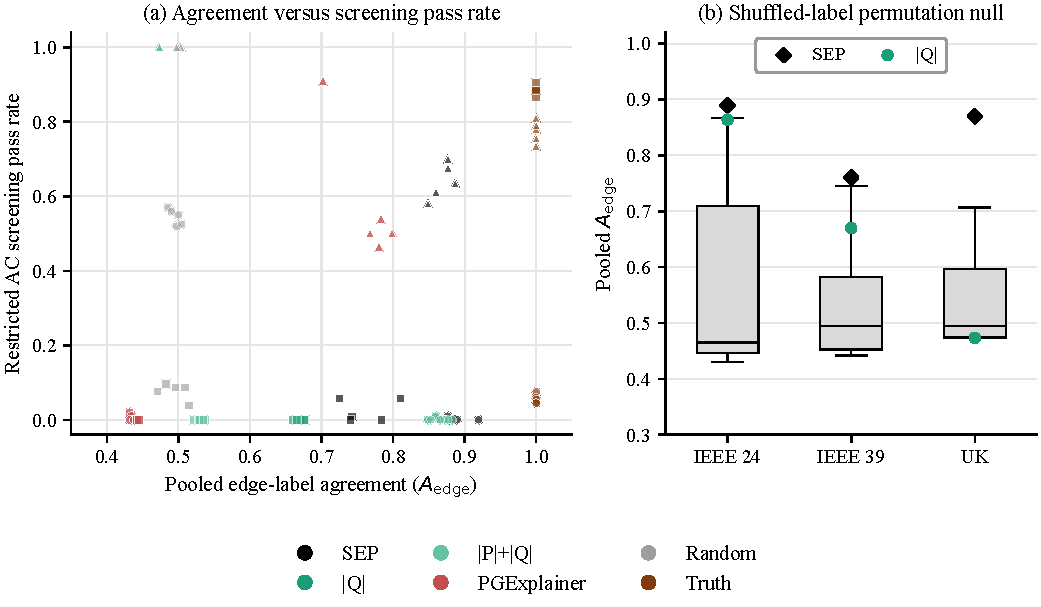
\includegraphics[width=\textwidth]{figures/figure_3_quality.pdf}
\caption{Edge-label agreement versus restricted AC screening pass rate. (a) Pooled edge BACC against screening pass rate for every method-system-seed observation, including the SEP, PGExplainer, the label-free $|Q|$ and $|P|+|Q|$ rankings, random edges, and the truth anchor. Marker shape denotes the system (circle = IEEE 24, square = IEEE 39, triangle = UK) and colour denotes the ranking family. (b) Permutation null for pooled edge BACC: classifiers trained on shuffled labels with the same split and features (ten permutations per seed, pooled over the five seeds); the observed SEP and $|Q|$ agreement values are marked (black diamonds: SEP; green dots: $|Q|$). The observed values are compared with this feature-specific null. The by-system correlations in Section~\ref{explanation_quality_does_not_substitute_for_raw_ac_operability} are descriptive, not inferential.}
\label{fig:quality}
\end{figure}



\subsection{Raw interventions fail through different physical mechanisms}\label{raw_interventions_fail_through_different_physical_mechanisms}

Table~\ref{tab:outcomes} consolidates the raw top-5 outcomes for all methods and systems on the matched slice. The table includes the pooled PFR, its cluster-bootstrap interval, the mean difference from the method's own matched random control, the paired effect size, and the failure counts. Edge-label agreement is not included because the archived per-edge rankings for GNNExplainer, Grad-CAM, GSAT, and SubgraphX are aggregate; Table~\ref{tab:quality} reports agreement only for the methods for which a per-edge ranking is available, and we do not impute missing values. Figure~\ref{fig:outcomes} shows the same rates with visible intervals and the failure taxonomy.

On IEEE 24, raw top-5 deletions pass the screen at 39.4\% for GNNExplainer, 0.6\% for PGExplainer, 9.5\% for Grad-CAM, 8.2\% for GSAT, and 4.5\% for SubgraphX; the random control passes at 54.5\% and the truth anchor at 5.6\%. The SEP passes at 0.2\%. Islanding and voltage violations are both common: GNNExplainer records 253 islands, 221 non-convergences, and 132 voltage violations in 1000 samples; the SEP records 458 islands, 226 non-convergences, and 314 voltage violations in 1000 matched samples. On IEEE 39 the screen is much more restrictive. GNNExplainer passes 0.96\%, PGExplainer 0.0\%, Grad-CAM 2.7\%, GSAT 0.0\%, and SubgraphX 4.8\%; random passes 7.7\% and the truth anchor 88.5\%. Islanding dominates the learned methods (471/520 for GNNExplainer, 478/520 for the SEP), but non-convergence is far from absent: PGExplainer records 384 non-convergences in 520 samples. On UK the screen is permissive for several methods: GNNExplainer passes 99.3\%, Grad-CAM 81.9\%, GSAT 100\% (one seed), SubgraphX 96.0\% (50 graphs), and the SEP 64.0\%; PGExplainer passes 58.2\% and random 100\%.

No overload failures are counted because thermal loading is not a rejection condition of the screen. This is why the table has no overload column: a zero column would suggest that overload was tested and absent, when in fact it was recorded and deliberately excluded. The public cases contain design-specific baseline overloads that would otherwise dominate the taxonomy.

The three failure categories are mutually exclusive by construction. Islanding indicates a loss of connectivity and is, in principle, repairable by choosing a different edge set. Non-convergence indicates that the nonlinear solver could not recover a solution under the declared initialization and iteration limit; it is a solver outcome and not proof of physical infeasibility. Voltage violation indicates that a converged solution exists but violates the declared interval. The connectivity-preserving control in Section~\ref{connectivity_control} separates the first mechanism from the other two. For the rankings with per-instance voltage detail, the severity-weighted risk in Eq.~\eqref{eq:risk} is 0.532 (GNNExplainer), 0.400 (random), and 0.680 (truth anchor) on IEEE 24; 0.990, 0.910, and 0.115 on IEEE 39; and 0.005, 0.000, and 0.226 on UK. These values are consistent with the taxonomy and are not imputed for methods without the required per-instance records.

\begin{table*}[!htbp]
\centering
\caption{Consolidated raw top-5 outcomes under the public-case restricted AC screen. PFR is the pooled screening pass rate over all audited samples; the interval is a seed-cluster bootstrap (2000 replicates). $\Delta$PFR is the mean paired difference from the method's own matched random control; the interval is a seed bootstrap. $d$ is the paired seed-level Cohen's $d$; $A_{\mathrm{edge}}$ is pooled edge-label agreement; ``--'' indicates that the quantity is not estimable from the available seeds or that the archived per-edge ranking is aggregate and the value is not recomputed. Denominators are not equal across methods and are shown as $n$. The main table is a benchmark under the random-split GIN backbone, not a fully held-out backbone-generalisation test; the footnote records the held-out status.}
\label{tab:outcomes}
\scriptsize
\resizebox{\textwidth}{!}{%
\begin{tabular}{llrrrcrcrrr}
\toprule
System & Method & Seeds & $n$ & PFR [95\% CI] & $\Delta$PFR [95\% CI] & $d$ & $A_{\mathrm{edge}}$ & Island & Non-conv. & Voltage \\
\midrule
\multirow{10}{*}{IEEE 24} & Random & 5 & 1000 & 0.545 [0.528, 0.562] & -- & -- & 0.491 & 207 & 121 & 127 \\
 & GNNExplainer & 5 & 1000 & 0.394 [0.372, 0.419] & $-0.157$ [-0.185, -0.129] & $-4.34$ & -- & 253 & 221 & 132 \\
 & PGExplainer & 5 & 1000 & 0.006 [0.000, 0.014] & $-0.545$ [-0.576, -0.514] & $-13.57$ & 0.435 & 946 & 48 & 0 \\
 & Grad-CAM & 5 & 1000 & 0.095 [0.057, 0.139] & $-0.456$ [-0.497, -0.421] & $-9.23$ & -- & 661 & 212 & 32 \\
 & GSAT & 3 & 600 & 0.082 [0.000, 0.190] & $-0.450$ [-0.515, -0.380] & $-6.65$ & -- & 476 & 44 & 31 \\
 & SubgraphX & 1 & 200 & 0.045 [--] & $-0.470$ [--] & -- & -- & 184 & 7 & 0 \\
 & SEP & 5 & 1000 & 0.002 [0.000, 0.006] & $-0.543$ [-0.558, -0.527] & $-26.50$ & 0.900 & 458 & 226 & 314 \\
 & $|Q|$ ranking & 5 & 1000 & 0.002 [0.000, 0.006] & $-0.543$ [-0.558, -0.527] & $-26.50$ & 0.861 & 0 & 388 & 610 \\
 & $|P|+|Q|$ ranking & 5 & 1000 & 0.000 [0.000, 0.000] & $-0.545$ [-0.562, -0.528] & $-25.01$ & 0.867 & 920 & 77 & 3 \\
 & Truth anchor & 5 & 1000 & 0.056 [0.047, 0.066] & $-0.489$ [-0.509, -0.466] & $-17.37$ & 1.000 & 0 & 43 & 901 \\
\midrule
\multirow{10}{*}{IEEE 39} & Random & 5 & 520 & 0.077 [0.058, 0.090] & -- & -- & 0.495 & 416 & 62 & 2 \\
 & GNNExplainer & 5 & 520 & 0.010 [0.002, 0.019] & $-0.077$ [-0.102, -0.050] & $-2.22$ & -- & 471 & 44 & 0 \\
 & PGExplainer & 5 & 520 & 0.000 [0.000, 0.000] & $-0.087$ [-0.110, -0.058] & $-2.71$ & 0.442 & 136 & 384 & 0 \\
 & Grad-CAM & 5 & 520 & 0.027 [0.000, 0.058] & $-0.060$ [-0.104, -0.004] & $-0.94$ & -- & 490 & 11 & 5 \\
 & GSAT & 3 & 312 & 0.000 [0.000, 0.000] & $-0.087$ [-0.125, -0.038] & $-1.96$ & -- & 305 & 7 & 0 \\
 & SubgraphX & 1 & 104 & 0.048 [--] & $-0.048$ [--] & -- & -- & 93 & 6 & 0 \\
 & SEP & 5 & 520 & 0.025 [0.002, 0.048] & $-0.052$ [-0.075, -0.031] & $-1.82$ & 0.760 & 478 & 15 & 14 \\
 & $|Q|$ ranking & 5 & 520 & 0.000 [0.000, 0.000] & $-0.077$ [-0.090, -0.058] & $-3.41$ & 0.670 & 456 & 64 & 0 \\
 & $|P|+|Q|$ ranking & 5 & 520 & 0.000 [0.000, 0.000] & $-0.077$ [-0.090, -0.058] & $-3.41$ & 0.530 & 387 & 133 & 0 \\
 & Truth anchor & 5 & 520 & 0.885 [0.873, 0.896] & $+0.808$ [+0.783, +0.838] & $+22.86$ & 1.000 & 4 & 56 & 0 \\
\midrule
\multirow{10}{*}{UK} & Random & 5 & 1000 & 1.000 [1.000, 1.000] & -- & -- & 0.501 & 0 & 0 & 0 \\
 & GNNExplainer & 5 & 1000 & 0.993 [0.986, 0.999] & $-0.007$ [-0.014, -0.001] & $-0.84$ & -- & 0 & 5 & 2 \\
 & PGExplainer & 5 & 1000 & 0.582 [0.486, 0.753] & $-0.418$ [-0.514, -0.247] & $-2.26$ & 0.766 & 418 & 0 & 0 \\
 & Grad-CAM & 5 & 1000 & 0.819 [0.638, 0.973] & $-0.181$ [-0.362, -0.027] & $-0.85$ & -- & 130 & 51 & 0 \\
 & GSAT & 1 & 200 & 1.000 [--] & $+0.000$ [--] & -- & -- & 0 & 0 & 0 \\
 & SubgraphX & 1 & 50 & 0.960 [--] & $-0.040$ [--] & -- & -- & 2 & 0 & 0 \\
 & SEP & 5 & 1000 & 0.640 [0.603, 0.677] & $-0.360$ [-0.397, -0.323] & $-7.45$ & 0.870 & 318 & 42 & 0 \\
 & $|Q|$ ranking & 5 & 1000 & 1.000 [1.000, 1.000] & $+0.000$ [+0.000, +0.000] & -- & 0.473 & 0 & 0 & 0 \\
 & $|P|+|Q|$ ranking & 5 & 1000 & 1.000 [1.000, 1.000] & $+0.000$ [+0.000, +0.000] & -- & 0.473 & 0 & 0 & 0 \\
 & Truth anchor & 5 & 1000 & 0.774 [0.750, 0.796] & $-0.226$ [-0.248, -0.204] & $-7.67$ & 1.000 & 226 & 0 & 0 \\
\bottomrule
\end{tabular}}
\begin{flushleft}
\footnotesize
Counts are pooled over seeds. The displayed Random row is the control shared by the SEP, $|Q|$, $|P|+|Q|$, and the truth anchor. Each learned method's $\Delta$PFR uses its own matched random draw on the same sample and candidate-edge set: the pooled random PFR is 0.551/0.0865/1.000 for GNNExplainer, PGExplainer, and Grad-CAM; 0.532/0.0865/1.000 for GSAT; and 0.515/0.0962/1.000 for SubgraphX on IEEE 24/IEEE 39/UK, respectively. Thus the displayed Random row is not the denominator for every difference. $d$ is the paired seed-level Cohen's $d$; ``--'' indicates that the quantity is not estimable (fewer than two seeds or zero variance across seeds); for $A_{\mathrm{edge}}$, it also indicates that the archived per-edge ranking is aggregate and the value is not recomputed. PFR intervals for one-seed methods are not reported. For the held-out status: every evaluated graph is held out from SEP and PGExplainer training, but the main table is not fully held out from the random-split GIN backbone, and the main GSAT extractor was trained on a random subset of the full simulation set; \ref{appendix:heldout_random} reports the held-out-backbone replication for all six methods, including a GSAT extractor retrained on non-test graphs. The SEP and $|Q|$ rows use the matched evaluation slice (Section~\ref{sample_selection}); the archived SEP at the earlier evaluation start is reported in Table~\ref{tab:matched}.
\end{flushleft}
\end{table*}

\begin{figure}[!htbp]
\makebox[\textwidth][c]{%
\begin{minipage}{1.15\textwidth}
\centering
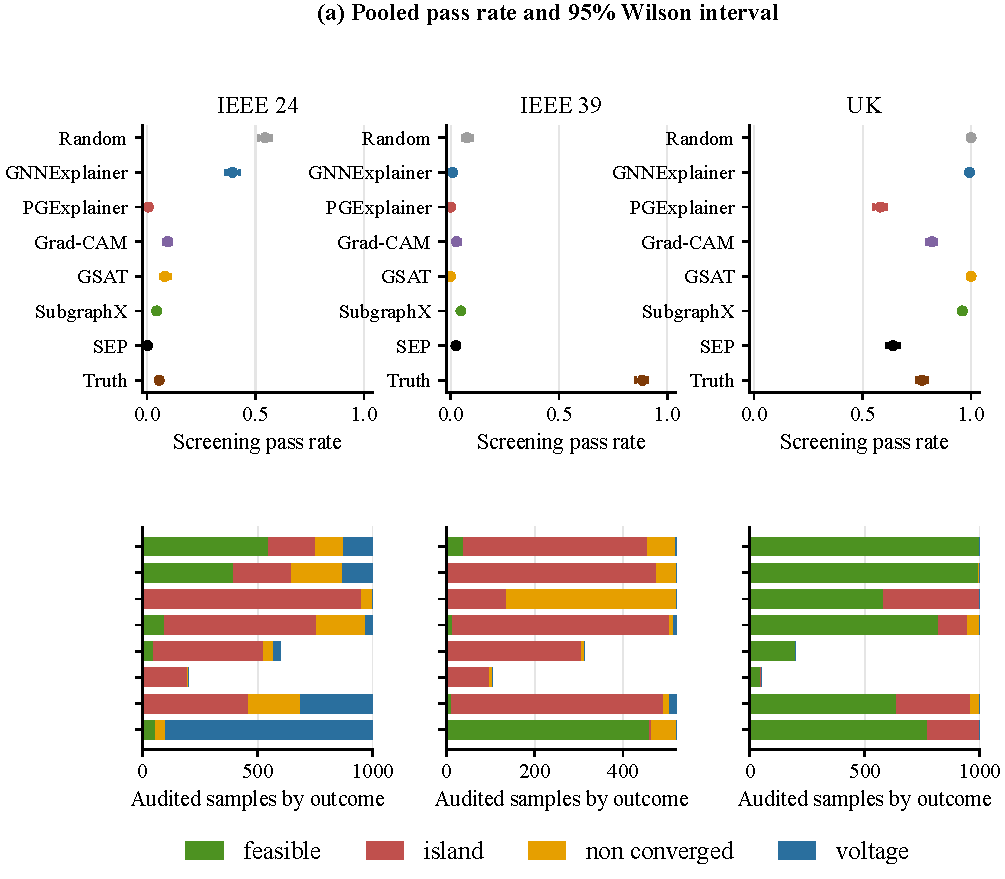
\includegraphics[width=\linewidth]{figures/figure_2_outcomes.pdf}
\caption{Raw top-5 interventions under the public-case restricted AC screen. (a) Pooled screening pass rate with 95\% Wilson intervals; the random row is the matched random control. Wilson intervals treat the pooled samples as independent and are drawn for display; the seed-cluster bootstrap interval for the same pass rate is the inferential interval and is reported in Table~\ref{tab:outcomes}. (b) Mutually exclusive failure taxonomy; bars sum to the audited samples. The figure includes the random control, the supervised SEP, and the learned rankings; the label-free $|Q|$ and $|P|+|Q|$ controls are shown in Figure~\ref{fig:quality}. Single-seed methods are shown without intervals. Thermal overload is not a rejection condition and is omitted.}
\label{fig:outcomes}
\end{minipage}}
\end{figure}



\subsection{Connectivity-preserving control separates islanding from AC-constrained failure}\label{connectivity_control}

The raw taxonomy does not separate failure by connectivity. We therefore construct a connectivity-preserving control: starting from the same SEP ranking, we accept a branch only if the joint deletion of all accepted branches leaves the bus graph connected. We scan the ranking until either $k=5$ connected branches are found or the ranking is exhausted; if fewer than five are found, the set is recorded as incomplete and counted as a screen failure. The screen is then evaluated exactly as in the raw protocol. 

Across five seeds, we audit 50 samples per seed per system (250 per system). On IEEE 24, only 1 of 250 raw top-5 sets passes the screen; 110 fail by islanding, 86 by voltage violation, and 53 by non-convergence. The connectivity-preserving control reaches five connected branches in all 250 samples, and only 1 of 250 connected sets passes; 187 fail by voltage violation and 62 by non-convergence. The raw failures therefore split into a topological component (110 samples) and an AC component that remains after connectivity is preserved. Even a connected five-edge deletion leaves the IEEE 24 case outside the voltage interval in almost every sample.

The other two systems behave differently. On IEEE 39, 6 of 250 raw sets pass and 232 fail by islanding; the connectivity-preserving control passes in 133 of 250 samples (53.2\%), with 20 non-convergences and 97 voltage violations remaining. On UK, 159 of 250 raw sets pass (63.6\%) and 84 fail by islanding; the connectivity-preserving control passes in 243 of 250 samples (97.2\%), with 7 non-convergences remaining. The connected-set pass rate is 0.4\% on IEEE 24, 53.2\% on IEEE 39, and 97.2\% on UK, with residual non-convergence and voltage failures, mainly on IEEE 39. Table~\ref{tab:conn} reports the complete breakdown. The control is pooled over five seeds and is reported as a mechanism check; it is not a substitute for the primary public-case table.

\begin{table}[!htbp]
\centering
\caption{Connectivity-preserving control (five seeds, 50 samples per seed; 250 samples per system). Each sample is classified as feasible, island, non-converged, or voltage violation; the pass column and the three failure columns sum to $n$. The connected rows use a five-edge set selected from the same SEP ranking under joint connectivity. The connected set reached five edges in 250/250 samples for every system.}
\label{tab:conn}
\scriptsize
\resizebox{\linewidth}{!}{%
\begin{tabular}{llrrrrr}
\toprule
System & Phase & $n$ & PFR & Island & Non-conv. & Voltage \\
\midrule
\multirow{2}{*}{IEEE 24} & Raw & 250 & 0.004 & 110 & 53 & 86 \\
 & Connected & 250 & 0.004 & 0 & 62 & 187 \\
\midrule
\multirow{2}{*}{IEEE 39} & Raw & 250 & 0.024 & 232 & 6 & 6 \\
 & Connected & 250 & 0.532 & 0 & 20 & 97 \\
\midrule
\multirow{2}{*}{UK} & Raw & 250 & 0.636 & 84 & 7 & 0 \\
 & Connected & 250 & 0.972 & 0 & 7 & 0 \\
\bottomrule
\end{tabular}}
\begin{flushleft}
\footnotesize
The connected set is selected by scanning the SEP ranking and accepting an edge only if the joint deletion of all accepted edges leaves the bus graph connected. A set that cannot reach five edges is counted as a screen failure; none occurred in these runs.
\end{flushleft}
\end{table}



\subsection{Matched samples and denominator checks}\label{matched_samples}

Table~\ref{tab:matched} compares the SEP and the matched random control on two evaluation slices. On IEEE 39, the earlier slice starts at index 20 and contains 134 graphs per seed; the matched slice starts at index 50 and contains 104 graphs per seed. On the matched 104-graph slice the SEP passes the screen in 2.5\% of samples (13/520) and the matched random control in 7.7\% (40/520); on the 134-graph slice the corresponding values are 2.4\% (16/670) and 8.5\% (57/670). The SEP pass rate remains below the matched random control on both slices, and both remain far below the truth anchor (88.5\%). The matched slice is used for all main comparisons; the 134-graph result is retained as a sensitivity analysis.

The same check applies to IEEE 24 and UK. On IEEE 24 the earlier SEP slice started at index 20 and passed in 0.3\% of 1000 samples; the matched slice starts at 50 and passes in 0.2\% of 1000 samples, while random passes in 54.5\%. On UK the earlier slice passed in 62.9\% of 1000 samples and the matched slice in 64.0\%, against 100\% for random. The edge-label agreement values also change only slightly between the per-graph and pooled definitions: the per-graph SEP values are 0.915/0.810/0.876 on IEEE 24/39/UK, while the pooled values are 0.900/0.760/0.870. The per-graph values average over graphs with no positive edge; the revision reports pooled values.

All evaluated graphs are held out from the SEP and PGExplainer training sets. They are not guaranteed to be held out from the GIN backbone's random training split; Section~\ref{sample_selection} states this limitation and the contingency-disjoint experiment addresses the prediction side. The exact indices, including the 30-graph purge gap between training and evaluation, are in \texttt{mapping/results\_split\_indices.json}.

\begin{table}[!htbp]
\centering
\caption{Effect of the evaluation-start choice on the IEEE 39 SEP comparison, with the corresponding IEEE 24 and UK checks. PFR is the restricted AC screening pass rate. The matched slice is used in all main tables.}
\label{tab:matched}
\scriptsize
\resizebox{\linewidth}{!}{%
\begin{tabular}{llrrrr}
\toprule
System & Slice & $n$/seed & SEP PFR & Random PFR & SEP $A_{\mathrm{edge}}$ \\
\midrule
IEEE 39 & start 20 (earlier) & 134 & 0.024 & 0.085 & 0.810 (per-graph) \\
IEEE 39 & start 50 (matched) & 104 & 0.025 & 0.077 & 0.760 (pooled) \\
IEEE 24 & start 20 (earlier) & 200 & 0.003 & 0.530 & 0.915 (per-graph) \\
IEEE 24 & start 50 (matched) & 200 & 0.002 & 0.545 & 0.900 (pooled) \\
UK & start 20 (earlier) & 200 & 0.629 & 1.000 & 0.876 (per-graph) \\
UK & start 50 (matched) & 200 & 0.640 & 1.000 & 0.870 (pooled) \\
\bottomrule
\end{tabular}}
\begin{flushleft}
\footnotesize
The per-graph agreement values average per-graph balanced accuracy over graphs, including graphs with no positive edge; the pooled values use Eq.~\eqref{eq:bacc} over all edges.
\end{flushleft}
\end{table}



\subsection{Prediction transfer under contingency-disjoint splits}\label{contingency_disjoint_evaluation_exposes_system_dependent_prediction_transfer}

Random graph splits yielded high GIN test BACC on all three systems, but contingency-disjoint testing changed both the level and variability of prediction performance (Figure~\ref{fig:transfer}; Table~\ref{tab:transfer}). Mean BACC decreased from 0.970 to 0.836 on IEEE 24 and from 0.926 to 0.731 on IEEE 39. The corresponding standard deviations increased from 0.010 and 0.035 to 0.101 and 0.175. Individual IEEE 39 seeds ranged from 0.540 to 0.927. UK remained high at $0.990\pm0.014$. Random-split BACC was therefore higher than contingency-disjoint BACC on IEEE 24 and IEEE 39, and similar on UK.

The intervals in Table~\ref{tab:transfer} are $t$-based intervals for the five observed seeds, computed on the logit scale and back-transformed to the BACC scale so that they remain inside $[0,1]$. They describe seed variation, not sampling uncertainty over contingencies. The test-scenario counts (6--9 per seed for IEEE 24 and IEEE 39, 13--27 for UK) show why the IEEE 39 interval is wide: several seeds evaluate only a handful of held-out contingencies. We therefore report the seed-level values in Figure~\ref{fig:transfer} rather than relying on the mean alone.

The contingency-disjoint split also permits a held-out audit of the SEP: the scorer is trained on some initiating contingencies and evaluated on disjoint ones, and the same public-case screen is applied. \ref{appendix:heldout} reports the result. On IEEE 24 the SEP passes in 0 of 1000 held-out samples and random in 51.9\%; on UK the SEP passes in 53.0\% and random in 100\%. On IEEE 39 the SEP passes in 17.3\% and random in 8.3\%, but the seed values range from 0\% to 55\%; the public-case ordering does not hold on this system. The SEP's absolute screening rate remains below the truth anchor on all three systems (7.3\%, 96.5\%, and 74.4\%).

To test whether the explanation audit can be performed on graphs the backbone never saw, we reconstructed the exact 10\% GIN random-test partition (the same ``torch.randperm'' split used in training) and reran all six explanation methods on it (\ref{appendix:heldout_random}): GNNExplainer, PGExplainer, Grad-CAM, GSAT, SubgraphX, and the SEP. The SEP and PGExplainer were trained only on non-test graphs; the GSAT extractor was retrained on 500 non-test graphs with the same 100-epoch configuration. The held-out audit gives the following pass rates. On IEEE 24 the six methods pass in 38.0\%, 2.0\%, 6.0\%, 4.0\%, 0.0\%, and 0.0\%, against 70.0\% for random and 4.0\% for the truth anchor. On IEEE 39 they pass in 0.0\%, 0.0\%, 0.0\%, 0.0\%, 6.3\%, and 0.0\%, against 18.8\% for random and 87.5\% for the truth anchor. On UK they pass in 100.0\%, 44.0\%, 96.0\%, 100.0\%, 96.0\%, and 42.0\%, against 100.0\% for random and 74.0\% for the truth anchor. The held-out partition contains no graph used to train the backbone, and none of its samples was used to train the SEP, PGExplainer, or GSAT extractor. GNNExplainer, Grad-CAM, and SubgraphX are post-hoc or training-free explanations on the frozen test-partition backbone. Table~\ref{tab:heldout_random} reports the complete held-out comparison.

\begin{table}[!htbp]
\centering
\caption{Predictive performance under random and contingency-disjoint graph splits. Values are mean $\pm$ SD over seeds 2--6. The interval is a two-sided 95\% $t$ interval with four degrees of freedom computed on the logit scale and back-transformed; it describes the five observed seeds, not a population interval over contingencies, and remains inside $[0,1]$.}
\label{tab:transfer}
\scriptsize
\resizebox{\linewidth}{!}{%
\begin{tabular}{lcccc}
\toprule
System & Random-split GIN BACC & Contingency-disjoint GIN BACC & 95\% $t$ interval & Test scenarios/seed \\
\midrule
IEEE 24 & $0.970\pm0.010$ & $0.836\pm0.101$ & 0.690--0.943 & 6--9 \\
IEEE 39 & $0.926\pm0.035$ & $0.731\pm0.175$ & 0.470--0.928 & 6--9 \\
UK & $0.971\pm0.003$ & $0.990\pm0.014$ & 0.971--0.999 & 13--27 \\
\bottomrule
\end{tabular}}
\end{table}

\begin{figure}[!htbp]
\centering
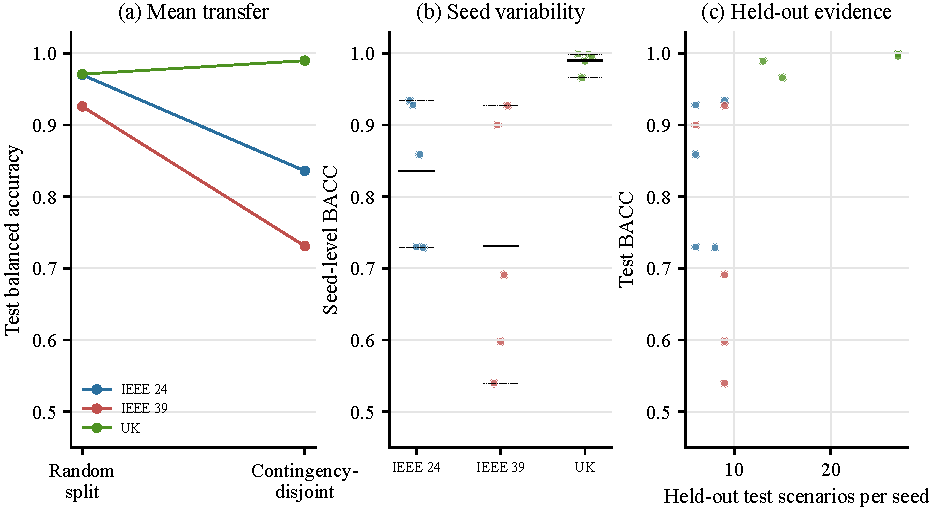
\includegraphics[width=\textwidth]{figures/figure_4_transfer.pdf}
\caption{Predictive performance under random and contingency-disjoint splits. (a) Test balanced accuracy under the two split protocols; paired lines connect reported means across protocols, not matched samples. (b) Seed-level stability under the contingency-disjoint protocol; filled markers are individual seeds, the solid bar is the seed mean, and the dotted lines are the seed minimum and maximum. (c) Held-out test evidence: test BACC against the number of held-out scenarios per seed; colour denotes system as in (a). IEEE 39 has the largest drop ($0.926\to0.731\pm0.175$) and the widest seed range; UK remains near its random-split level.}
\label{fig:transfer}
\end{figure}



\subsection{Screening rates under changes in budget, threshold, and operating state}\label{operability_is_sensitive}

Figure~\ref{fig:protocol} and Table~\ref{tab:protocol} report the protocol sensitivity. The SEP screening rate falls sharply with the intervention budget on IEEE 39 and UK: 1.000 at $k=1$, 0.192 at $k=3$, 0.010 at $k=5$, and 0.000 at $k=8$ on IEEE 39; 1.000 at $k=1$ and $k=3$, 0.700 at $k=5$, and 0.055 at $k=8$ on UK. On IEEE 24 the SEP is at 0.000 for every $k$, while the random control falls from 0.975 at $k=1$ to 0.520 at $k=5$ and 0.170 at $k=8$. The screening rate varies with $k$ in every system; the choice of $k$ is therefore part of the reported protocol.

Stricter voltage thresholds change the random control much more than the SEP. On IEEE 39 the SEP rate is 0.010 at 0.85, 0.90, and 0.95 p.u.; the random control falls from 0.087 to 0.067 to 0.029. On IEEE 24 both are at or near zero for the SEP, while random falls from 0.520 to 0.320 to 0.005. On UK the SEP is 0.700 at all three thresholds, while random falls from 1.000 to 1.000 to 0.990. The SEP rate is unchanged across the three thresholds in every system, whereas the random rate falls with stricter thresholds on IEEE 24 and IEEE 39.

DC and AC screening rates differ (Table~\ref{tab:protocol}). On IEEE 24 the SEP's DC rate is 0.510 while its AC rate is 0.000; the truth anchor's DC rate is 1.000 while its AC rate is 0.075. DC and AC rates differ by 0.510 on IEEE 24, 0.000 on IEEE 39, and 0.010 on UK. IEEE 39 is restrictive under both formulations, and UK is close across AC and DC.

The operating-point comparison uses the same raw top-$k$ sets under both protocols. On IEEE 24 the raw SEP set passes in 0.0\% of samples under the public case and 0.0\% under the sample-conditioned case; the reconstructed base state passes in 97.0\%. On IEEE 39 the public rate is 1.0\% and the sample-conditioned rate is 0.0\% (base 88.5\%); on UK the public rate is 70.0\% and the sample-conditioned rate is 8.0\% (base 100.0\%). The sample-conditioned protocol therefore changes the level substantially, but it does not reverse the public-case ordering: the SEP remains below the random control in all three systems (public/sample SEP versus random: 0.0\%/0.0\% versus 52.0\%/46.0\% on IEEE 24; 1.0\%/0.0\% versus 8.7\%/1.0\% on IEEE 39; and 70.0\%/8.0\% versus 100.0\%/100.0\% on UK). The observed deletion rates do not exceed the reconstructed base rate in these runs, but this is an empirical pattern, not a cap: a topology change can in principle restore feasibility, and the screen does not exclude such cases.

\begin{table}[!htbp]
\centering
\caption{Protocol sensitivity of the restricted AC screening pass rate (seed 2 unless stated; $n=200/104/200$ for IEEE 24/IEEE 39/UK in each row). Top: intervention budget and voltage threshold. Bottom: DC versus AC and public versus sample-conditioned operating states, evaluated on identical raw top-5 sets; the base columns are the empty-set audit, not a top-5 deletion.}
\label{tab:protocol}
\scriptsize
\resizebox{\linewidth}{!}{%
\begin{tabular}{lcccccc}
\toprule
\multirow{2}{*}{System} & \multicolumn{4}{c}{SEP PFR by $k$ (0.85 p.u.)} & \multicolumn{2}{c}{SEP PFR at $k=5$} \\
\cmidrule(lr){2-5}\cmidrule(lr){6-7}
 & $k=1$ & $k=3$ & $k=5$ & $k=8$ & 0.90 p.u. & 0.95 p.u. \\
\midrule
IEEE 24 & 0.000 & 0.000 & 0.000 & 0.000 & 0.000 & 0.000 \\
IEEE 39 & 1.000 & 0.192 & 0.010 & 0.000 & 0.010 & 0.010 \\
UK & 1.000 & 1.000 & 0.700 & 0.055 & 0.700 & 0.700 \\
\midrule
\multirow{2}{*}{System} & \multicolumn{2}{c}{AC vs DC (SEP)} & \multicolumn{2}{c}{Public vs sample (raw SEP)} & \multicolumn{2}{c}{Base control} \\
\cmidrule(lr){2-3}\cmidrule(lr){4-5}\cmidrule(lr){6-7}
 & AC & DC & Public & Sample & Public & Sample \\
\midrule
IEEE 24 & 0.000 & 0.510 & 0.000 & 0.000 & 1.000 & 0.970 \\
IEEE 39 & 0.010 & 0.010 & 0.010 & 0.000 & 1.000 & 0.885 \\
UK & 0.700 & 0.710 & 0.700 & 0.080 & 1.000 & 1.000 \\
\bottomrule
\end{tabular}}
\begin{flushleft}
\footnotesize
All values are single-seed (seed 2) sensitivity results, not five-seed estimates. The $k$ and threshold columns use raw top-$k$ sets; the operating-point columns use the same raw top-5 set under both protocols and no wrapper. The public base is the empty-set public case; the sample base is the reconstructed state with the initiating outage retained. The corresponding public/sample random rates are 52.0\%/46.0\% on IEEE 24, 8.7\%/1.0\% on IEEE 39, and 100\%/100\% on UK.
\end{flushleft}
\end{table}

\begin{figure}[!htbp]
\centering
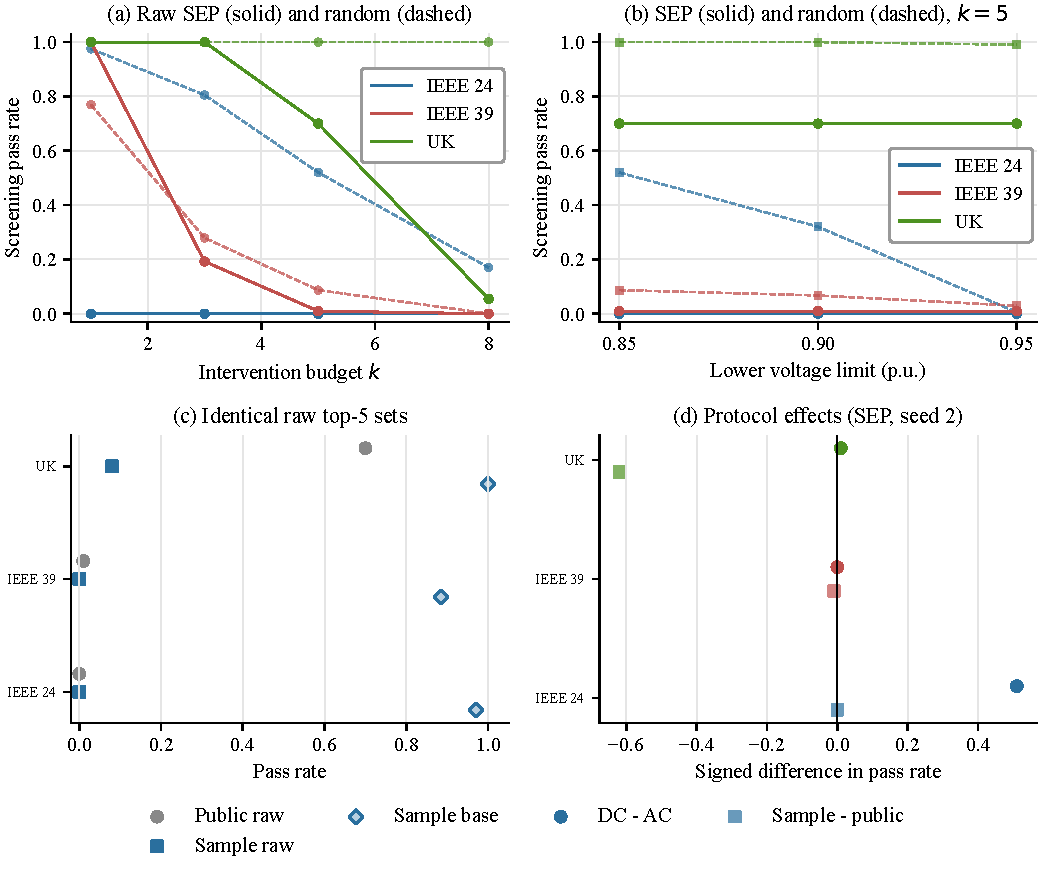
\includegraphics[width=\textwidth]{figures/figure_5_protocol.pdf}
\caption{Screening pass rate under different intervention budgets, voltage thresholds, and operating states. (a) Raw SEP screening pass rate for $k=1,3,5,8$ at 0.85 p.u., with the matched random control. (b) Raw SEP and random screening rates at 0.85, 0.90, and 0.95 p.u. for $k=5$. Colours denote systems in (a) and (b). (c) Identical raw top-5 sets audited under the public and sample-conditioned protocols, with the reconstructed base rate shown as a separate marker. (d) DC minus AC and sample-minus-public signed differences. All panels are seed-2 sensitivity results on the $n=200/104/200$ IEEE 24/IEEE 39/UK slices; neither DC nor sample-conditioned reconstruction replaces the primary public-case AC screen.}
\label{fig:protocol}
\end{figure}



\subsection{Feasibility repair changes the explanation and has a measurable AC cost}\label{wrapper_changes_explanation}

The local-swap wrapper restores screening feasibility in all five-seed runs: the wrapped PFR is 1.000 for the SEP on IEEE 24, IEEE 39, and UK, and the incomplete count is zero. Table~\ref{tab:wrapper} reports the wrapped PFR, the replacement rate, and the AC-call distribution. The wrapper rewrites a fraction of the selected edge set: $0.283\pm0.082$ on IEEE 24, $0.276\pm0.078$ on IEEE 39, and $0.074\pm0.009$ on UK. On IEEE 24 this means that, on average, more than one of the five edges is replaced; on UK the replacement rate is smaller (0.074).

Because the wrapper rewrites part of the selected set, the wrapped set is a different intervention from the raw explanation. We therefore do not treat its label agreement as a repaired version of the raw agreement or pool the two; the wrapped evidence is reported separately as wrapped PFR, replacement rate, and AC-call cost. 

The AC-call bound is larger than the commonly quoted $kP=40$ bound. That bound counts only the local-swap replacements: $k=5$ and $P=8$ give at most 40 audits. The greedy phase also audits candidates until it has accepted five feasible edges, and it can scan many more than five. On the same seed-2, first-20-graph workload used for the runtime benchmark, the wrapper used a mean of 21.8 AC evaluations per graph on IEEE 24, with a median of 21, a maximum of 29, and 90th/95th percentiles of 22/23; on IEEE 39 the mean, median, maximum, and 90th/95th percentiles are 27.1, 29, 31, and 30/30; on UK they are 20.2, 20, 21, and 21/21. The count excludes the initial empty-set base audit and assumes the single local-swap round in Algorithm~\ref{alg:wrapper}. The correct worst-case bound is therefore $N_{\mathrm{avail}}+kP$, where $N_{\mathrm{avail}}$ is the number of available branches, not $kP$ alone. We report the measured distribution rather than a single bound.

\begin{table}[!htbp]
\centering
\caption{Finite-budget wrapper cost (SEP, five seeds for PFR and replacement rate; seed 2, first 20 samples, for the AC-call distribution, matching the runtime workload). ``Replace'' is the fraction of the five-edge set rewritten by the wrapper. ``AC calls'' counts every AC power-flow evaluation in the greedy and local-swap phases; it excludes the initial empty-set base audit and assumes the single swap round in Algorithm~\ref{alg:wrapper}.}
\label{tab:wrapper}
\scriptsize
\resizebox{\linewidth}{!}{%
\begin{tabular}{lrrrrrrrr}
\toprule
System & Wrapped PFR & Replace rate & AC calls mean & Median & Max & p90 & p95 & Incomplete \\
\midrule
IEEE 24 & 1.000 & $0.283\pm0.082$ & 21.8 & 21 & 29 & 22 & 23 & 0/5 \\
IEEE 39 & 1.000 & $0.276\pm0.078$ & 27.1 & 29 & 31 & 30 & 30 & 0/5 \\
UK & 1.000 & $0.074\pm0.009$ & 20.2 & 20 & 21 & 21 & 21 & 0/5 \\
\bottomrule
\end{tabular}}
\begin{flushleft}
\footnotesize
The wrapper is a constrained search, not an explanation method. Wrapped PFR describes the repaired set; the replacement rate quantifies how much of the explanation was rewritten. Wrapped and raw outcomes are never pooled.
\end{flushleft}
\end{table}



\subsection{Backbone and fidelity checks}\label{backbone_fidelity_results}

\ref{appendix:backbone} reports a reduced Transformer-backbone check (three seeds, 50 graphs per run). The Transformer results are: on IEEE 24 the Transformer GNNExplainer passes in 0.487 of samples versus 0.600 for random; on IEEE 39 it passes in 0.060 versus 0.073 for random; on UK it passes in 0.953 versus 1.000 for random. The Transformer check is a pilot, not a five-seed replication, and it does not support a backbone-independent claim.

\ref{appendix:fidelity} reports the fidelity check. The GNNExplainer check (seed 4, 50 graphs) preserves the graph prediction in 100\% of cases when the top-5 edges are retained, while deleting them flips the prediction in 6\%. The GSAT check (seed 3, 10 graphs) gives 100\% and 10\%. 

\section{Discussion}\label{discussion}

The four answers share a common structure. The SEP has the highest edge-label agreement among the non-truth rankings in every system, yet its screening pass rate is lower than the matched random control. The raw failures are mechanism-specific, with islanding, non-convergence, and voltage violations appearing in different proportions. The ordering is sensitive to the evaluation slice, the split, the intervention budget, and the operating state. The wrapper restores feasibility only by rewriting part of the explanation. The remainder of this section places these results in dialogue with prior work (Section~\ref{discussion_literature}), proposes a mechanism for the pattern (Section~\ref{discussion_mechanism}), and identifies observations that the mechanism does not yet explain (Section~\ref{discussion_unexpected}).

\subsection{Dialogue with prior work}\label{discussion_literature}

\textbf{Agreement with the explanation literature.} Our first layer is consistent with the critique of post-hoc explanation, but it locates the failure at a different point. Adebayo et al.~\citep{adebayo2018} showed that some saliency maps are largely insensitive to model parameters and can still appear plausible; our permutation null shows a complementary phenomenon. A ranking can score highly against a label because the label is concentrated on a feature subspace, even when the ranking carries no edge-level information. Hooker et al.~\citep{hooker2019} and Samek et al.~\citep{samek2017} established that fidelity is a model-internal property; our $\mathrm{Fid}^{+}=100\%$ and $\mathrm{Fid}^{-}=6\%$ reproduce their caution that retaining and deleting features are not symmetric tests, and we add that both can coexist with a zero screening rate. Jacovi and Goldberg~\citep{jacovi2020} distinguish plausibility from faithfulness; edge-label agreement is a plausibility metric in their sense, and our results provide a physical-domain demonstration that plausibility does not imply operational validity. The survey of Yuan et al.~\citep{yuan2022} documents that GNN explanation evaluation lacks a unified protocol; we do not claim a universal protocol, but we show what a domain-specific one must separate. Our reading of Rudin~\citep{rudin2019} is similar but narrower: the results support her argument that post-hoc explanations are insufficient for high-stakes decisions, yet they do not imply that post-hoc methods are useless. They imply that a post-hoc explanation needs an external validity layer before it is used for action.

\textbf{Contradiction with the cascade-explanation assumption.} The results contradict a specific inferential step in the cascade-explanation literature, not the explainers themselves. PowerGraph and related studies provide simulator cascade-path masks as edge-level explanation labels, and agreement with those masks is commonly read as evidence that an explanation is meaningful~\citep{varbella2024}. Our results show that this inference is not licensed. A label-free $|Q|$ ranking reaches 0.861 pooled BACC on IEEE 24, close to the SEP's 0.900, and shuffled-label classifiers can reach 0.866; yet the $|Q|$ and SEP rankings pass the AC screen in 0.2\% of samples. The masks remain valid labels for what the simulator propagated; they are not labels for what can be switched. This is the point at which our work departs from the benchmark's implicit validation logic, and it is the main reason the audit layer is necessary.

\textbf{Relation to corrective switching.} The power-system literature has long required corrective switching to be AC-feasible and operating-point aware~\citep{rolim1999,li2019,korad2013,li2017}. We do not contradict that literature; we show that explanation rankings, when treated as switching candidates, violate its central constraint at rates that are substantial on IEEE 24 and IEEE 39. The contribution is therefore not a new switching optimizer but a bridge. We subject the ranking an explainer produces to the same feasibility logic that corrective switching already uses, and we quantify the gap between label agreement and physical feasibility.

\textbf{Relation to physics-informed learning.} Physics-informed learning embeds conservation laws or simulator constraints in training~\citep{misyris2020,xu2023}. Our results suggest that this is complementary to, not a substitute for, a physical evaluation layer. A physics-informed predictor would still be exposed to the same post-hoc layer: the explanation is generated after training and is not constrained by the AC state. The distinction is between physics in the model and physics in the audit.

\subsection{A mechanism for the agreement--operability gap}\label{discussion_mechanism}

We propose that the gap is generated by three mismatches. We call their composite the \emph{intervention gap}: the difference between what an explanation identifies and what a declared intervention can physically execute. The framework is a hypothesis, not a proven causal model; the experiments isolate each mismatch only partially.

\textbf{Label mismatch.} A cascade-path mask is a propagation label, generated by the simulated cascade, not by a switching decision. It is also a function of the post-contingency branch flows, which are input features of the predictor. A ranking that is correlated with flow magnitude can therefore score highly without encoding feasibility. The label-free $|Q|$ ranking and the shuffled-label classifiers are direct evidence for this channel: they reproduce much of the agreement while carrying no label or model information. The mismatch predicts that the agreement--operability gap should widen as the positive edges concentrate in a small feature subspace, for example the top flow decile.

\textbf{Model mismatch.} Explainers optimize a model-internal objective: a mask that preserves a prediction, a Shapley value, a gradient, or an attention score. None of these objectives contains the AC state, the switching sequence, or the operating point. An explanation can therefore be faithful to the classifier and still select a set that islands the network or violates voltage limits. The fidelity check is consistent with this channel: retaining the top edges preserves 100\% of predictions and deleting them flips only 6\%, while the same GNNExplainer ranking passes the screen in 39.4\% of IEEE 24 samples and the SEP, with the highest agreement, in 0.2\%. The mismatch predicts a weak relation between fidelity and PFR within a fixed system.

\textbf{State mismatch.} Explanations are computed on the post-contingency sample graph, in which the initiating outage branches have been removed. The physical screen applies the deletion to a declared operating case, which either restores the public topology and dispatch or reconstructs a sample-conditioned state. The mapping from one state to the other is not the identity. The same ranking can therefore pass under one protocol and fail under another; the IEEE 39 comparison (1.0\% under the public case versus 0.0\% under the sample-conditioned case) is an instance. The mismatch predicts that reversals are most likely when the base state is near the feasibility boundary.

These channels yield testable predictions. First, if the label mismatch dominates, the gap should increase with the feature concentration of the positive edges. Second, if the model mismatch dominates, fidelity and PFR should be weakly related within a system. Third, if the state mismatch dominates, the ordering should reverse when the operating point moves close to the feasibility boundary. Our experiments are consistent with all three, but they do not separate their relative contributions; doing so requires a design that holds two channels fixed while varying the third.

\subsection{Unexpected observations and open questions}\label{discussion_unexpected}

Five observations go beyond the framework above. We state them as open questions rather than conclusions, because each would require a separate study to establish its mechanism.

\textbf{The truth anchor is not uniformly the best intervention.} The truth anchor has perfect edge-label agreement by construction, but its screening rate is 5.6\% on IEEE 24 and 88.5\% on IEEE 39. If agreement were a sufficient validation, the truth anchor should also be the best intervention; it is best on IEEE 39 but far from best on IEEE 24. We do not have a complete explanation. A plausible one is that the mask encodes propagation, and on a voltage-limited network the propagated path contains branches whose removal is electrically destabilizing, whereas on a topology-limited network it approximates a cut set whose removal is feasible. This suggests that label validity is system-dependent, a hypothesis that can be tested by comparing the electrical role of mask edges across systems.

\textbf{Agreement and operability decouple in both directions.} On UK the label-free $|Q|$ ranking has chance-level agreement (0.473) but a 100\% screening rate, while the SEP has 0.870 agreement and 64.0\%. A tentative explanation is that the UK screen is permissive (the random control passes 100\%), so the pass rate is saturated and cannot discriminate rankings; the SEP's lower rate reflects its selection of higher-flow branches that are more likely to be voltage-critical. This predicts that the decoupling should disappear under a stricter screen or a less redundant network.

\textbf{The dominant failure mechanism is a system property.} On IEEE 24 a connectivity-preserving control still passes in only 1 of 250 samples, whereas on IEEE 39 and UK the connected-set pass rate rises to 53.2\% and 97.2\%. The same intervention logic produces opposite diagnoses: IEEE 24 is AC-limited even when connected, whereas IEEE 39 and UK are primarily topology-limited. This suggests a system-level classification, AC-limited versus topology-limited, that is a property of the network and the operating state rather than of the explainer. Network redundancy, load margin, and the distribution of branch flows are candidate predictors of that classification.

\textbf{DC screening can certify an AC-infeasible intervention.} On IEEE 24 the SEP's DC screening rate is 51.0\% while its AC rate is 0.0\%; the truth anchor is 100\% under DC and 7.5\% under AC. DC screening certifies active-power feasibility but is blind to voltage and convergence, so the difference is a direct measure of AC-only failure modes. This is consistent with the power-system literature, but to our knowledge it has not been quantified for explanation rankings. The observation matters because DC screening is often used as a cheap surrogate in contingency screening.

\textbf{Scenario-conditional effects can dominate method effects.} The held-out IEEE 39 SEP audit passes in 17.3\% of scenarios versus 8.3\% for random, with seed values from 0\% to 55\%. A single ``SEP below random'' claim does not survive this protocol. This is the clearest evidence that scenario-conditional effects can dominate method effects, and it motivates scenario-level rather than sample-level validation. It also cautions against treating a five-seed mean as a stable ranking when the seed-level range spans most of the unit interval.

Each observation is a candidate for a separate study. We report them because they are visible in the data and are not explained by the three-mismatch framework alone; treating them as noise would hide the most interesting boundary of the present design.

\subsection{Implications for explainable reliability assessment}\label{implications_for_explainable_reliability_assessment}

The results support a layered reporting standard. A model explanation should first be assessed for its relationship to the predictor (fidelity) or to an available process label (agreement). If the explanation is then interpreted as an intervention candidate, it should pass a separate physical screen at a declared operating state. Only after this screen should a system consider optimization, operator constraints, switching costs, or dynamic validation. A failed screen is a failure of the intervention candidate, not by itself a failure of the explanation's diagnostic value. This ordering keeps diagnostic explanation, counterfactual testing, and operational decision-making conceptually separate.

The standard should also report the denominator and the operating state. A screening rate conditional on accepted positive-class samples is not a rate over the risk population. A rate under a public case is not a rate at the sample-specific dispatch. A rate under a reconstructed base with 88.5\% base feasibility in IEEE 39 is not directly comparable with a rate under a public case with a feasible base. These quantities are separated here, and the base controls are reported. The lesson is not specific to this benchmark: any explanation-to-action study needs a declared intervention semantics, a declared state, and a denominator.

The wrapper result adds a reporting requirement. A wrapper that achieves a 100\% screening rate has not shown that the explanation is operable; it has shown that a constrained search can find a feasible set. The relevant quantities are how much of the explanation was rewritten, how many AC evaluations were consumed, and whether the search ever failed to reach $k$; where the modified set is rescored, the change in label agreement should also be reported. We report the first three and treat the agreement change as a property of the modified set rather than of the original explanation. A wrapper that rewrites 28\% of the edge set on IEEE 24 and 7\% on UK is doing materially different work in the two systems, and the difference should be visible to a reader.

\subsection{Scenario transfer and system heterogeneity}\label{scenario_transfer_is_part_of_reliability_evidence}

The contingency-disjoint experiment shows that standard random graph splits can conceal scenario dependence. IEEE 39 exhibited large seed-to-seed variation even though its random-split mean was high. This variation propagates into explanation studies because an explanation is conditional on the predictor and on the evaluated graph distribution. Reliability claims should therefore state whether operating points from the same initiating contingency can appear on both sides of a split.

UK behaved differently from IEEE 24 and IEEE 39 across several analyses. Its high scenario-aware prediction BACC and generally higher screening rate do not invalidate the failure observed in the smaller systems; they demonstrate system heterogeneity. Network redundancy, case construction, and operating-point characteristics can change the consequence of deleting the same number of ranked edges. A universal claim based on one system would therefore be inappropriate.

\subsection{Limitations}\label{limitations}

This study uses simulated PowerGraph data and three benchmark systems. It does not include an external utility dataset, operator-approved switching records, or real event replay. The public MATPOWER operating case is reproducible but does not represent the sample-specific pre-contingency dispatch. The sample-conditioned reconstruction is an approximation: it derives net injections from post-contingency branch flows, retains the initiating outage, and can produce a base state that is itself infeasible, especially in IEEE 24 and IEEE 39 (base feasibility 97.0\% and 88.5\%, respectively). It is a sensitivity analysis, not ground truth.

The screen is restricted. It checks convergence, connectivity, and voltage; it does not enforce thermal limits, generator reactive limits, transformer tap adjustments, redispatch, remedial action schemes, transient dynamics, protection coordination, switching sequence constraints, or operator rules. Non-convergence is treated as a screen failure, not as proof of physical infeasibility. The voltage interval is a declared N-1-style convention, not a utility-specific limit. The thermal channel is recorded but not used as a rejection condition because the source cases contain design-specific baseline overloads. A passing result is therefore evidence for the declared counterfactual only, not sufficient for an operational recommendation.

The three-mismatch framework is a hypothesis. The design isolates the label mismatch through the label-free and shuffled-label controls, and the state mismatch through the public-versus-sample-conditioned comparison, but the model mismatch is inferred from the fidelity check rather than manipulated. A direct test would hold the label and the operating state fixed and vary only the explainer objective. Until such a test is available, the relative contribution of the three channels remains an open question.

All formal explanation comparisons use one GIN backbone. Because that backbone was trained under a random graph split, the main table is not a fully held-out graph evaluation: some evaluated graphs may have appeared during backbone training. \ref{appendix:heldout_random} provides a held-out-backbone replication for all six methods (GNNExplainer, PGExplainer, Grad-CAM, GSAT, SubgraphX, and the SEP) on the exact GIN test partition, where no evaluated graph was used to train the backbone or the supervised components and the GSAT extractor was retrained only on non-test graphs. This held-out audit is seed-2 and covers 50/16/50 graphs; it is not a five-seed held-out evaluation, and the seed-2 evidence for GSAT and SubgraphX should be read with that caveat. The main GSAT extractor was trained on a random subset of the full simulation set and is not guaranteed to be held out from the main-table evaluation graphs; Appendix D retrains it on non-test graphs. The Transformer check is a three-seed pilot at 50 graphs per run and is reported in the appendix; it is not a five-seed replication and does not support a backbone-independent claim. Resource constraints also limited compatible GSAT seeds and the UK SubgraphX workload. Where a comparison could not be run compatibly, the affected quantities are reported as missing rather than replaced with incompatible results.

The IEEE 39 explainable-positive population contains only 154 graphs. The 104-graph evaluation slice covers most of that population, and the five seeds draw partially overlapping subsets. The reported intervals describe seed variation and do not account for the overlap. The IEEE 24 and UK populations are larger, but the accepted slices still overlap across seeds. None of the intervals is a population confidence interval over graphs or contingencies.

The contingency signature is a heuristic. It treats every branch with exactly zero post-contingency flow as part of the initiating outage; a branch can be at zero flow for other reasons, so the signature can merge contingencies that are not physically identical. The contingency-disjoint split is therefore a stress test of scenario dependence, not a verified outage reconstruction. A more precise outage list, if available, would sharpen the transfer experiment.

The wrapper is a local search, not an optimal repair. It uses a fixed candidate pool of eight edges and a one-edge swap; it does not explore multi-edge repairs, re-dispatch, or switching sequences. Its replacement rate is a measure of modification, not a measure of causal loss. A different wrapper could achieve feasibility with a smaller or larger modification, and the reported rates should be read as properties of this declared wrapper, not of feasibility repair in general.

Finally, the study does not include an LODF/PTDF or contingency-ranking baseline. The label-free flow-magnitude controls are deliberately simple and are used to test the metric, not to represent the state of the art in line-criticality ranking. A comparison with sensitivity-based and optimization-based criticality methods under the same locked screen is left to future work.

\subsection{Future work}\label{future_work}

The three-mismatch framework suggests a sequence of targeted tests. A feature-matched permutation null, in which the shuffled labels are constrained to preserve the feature distribution of the positive edges, would isolate the label channel from the explanatory signal. Holding the operating state fixed while varying the explainer objective would isolate the model channel. Moving the operating point toward the feasibility boundary in a controlled way would isolate the state channel. Each test is feasible with the present benchmark and would turn the framework from a post hoc interpretation into a falsifiable model.

Future validation should also combine explanation ranking with corrective-switching or security-constrained optimal power flow, include redispatch and reactive-power controls, and test dynamic cascade simulators. External validation should group events by operating regime and initiating contingency and should include true switching costs and operator constraints. A fully budget-matched multi-backbone comparison and complete N-2 sensitivity would establish whether the observed explanation--operability gap persists beyond the present GIN-centered benchmark.

On the metric side, the field needs explanation labels that are not simple functions of the input features, or evaluation designs that explicitly control for feature separability. A prospective test would generate explanations for held-out contingencies, apply the screen, and compare the screen outcome with operator-reviewed switching actions. None of these is available in the current benchmark.

\section{Conclusions}\label{conclusions}

This paper began from a validation practice that is widely used but rarely stated: an edge explanation is treated as validated when it agrees with a simulator cascade-path mask. The implicit assumption was that agreement certifies the explanation for intervention. The audit tests that assumption directly, and the answer is negative. Across IEEE 24, IEEE 39, and UK, a label-free reactive-flow ranking reaches pooled edge BACC close to the supervised edge-label predictor, shuffled-label classifiers reproduce much of the same agreement, and the non-truth rankings with the highest agreement pass the restricted AC screen less often than the matched random control. Agreement is a property of the label and the features; it is not a certificate of faithfulness or operability.

The result fills the gap identified in Section~\ref{introduction}. The explanation literature validates explanations with model-internal quantities, and the power-system literature requires switching to be AC-feasible, but post-switching AC feasibility was absent from both validation vocabularies. This work supplies that missing layer and makes it operational: the explanation is treated as a counterfactual topology intervention, the top-$k$ branches are removed from a declared operating case, and convergence, connectivity, and voltage are checked. Of the three barriers identified in Section~\ref{introduction}, the audit removes the evaluation barrier by providing a reproducible protocol; it mitigates the data barrier by reconstructing and disclosing the operating state and by releasing the exact splits and artefacts; it does not remove the methodological barrier, because explainers still do not optimize for AC feasibility. That boundary is part of the contribution: the protocol detects a gap that the explainer cannot close by itself.

The results also support a mechanism, which we offer as the paper's theoretical endpoint and as a hypothesis for future tests. We call the composite of the label, model, and state mismatches the \emph{intervention gap}: the difference between what an explanation identifies and what a declared intervention can physically execute. The label channel is feature confounding, the model channel is the absence of the AC state from explainer objectives, and the state channel is the mismatch between the explanation graph and the screened operating case. The framework explains why agreement and operability can diverge, and it yields testable predictions: the gap should widen with feature concentration, fidelity and PFR should be weakly related, and orderings should reverse near the feasibility boundary. It also leaves observations it does not yet explain---the system-dependent truth anchor, the UK decoupling, the AC-limited versus topology-limited classification, the DC/AC gap, and the held-out IEEE 39 reversal. We report them as open questions rather than as anomalies to be smoothed over.

The significance is both scientific and practical. Scientifically, the paper separates three quantities that were conflated and replaces a sufficiency claim with a measured gap and a mechanism. Practically, it gives a reporting standard that can be adopted without changing the explainer: report agreement as a label diagnostic, fidelity as a model check, the AC screen as a separate physical layer, and the wrapper as a modified intervention with a replacement rate, the wrapped screening rate, and an AC-call cost. The timing matters. GNNs are moving from benchmark prediction toward operational decision support, explainability is increasingly expected in high-stakes settings, and open cascade benchmarks together with open AC engines make a simulator-in-the-loop audit reproducible. The protocol is therefore available before explanation-based tools are widely deployed, which is the point at which a validation standard can still shape practice.

The conclusion is deliberately narrow. The evidence comes from simulated benchmark data, three systems, a restricted convergence--connectivity--voltage screen, one GIN backbone with a reduced Transformer pilot, and a local-search wrapper; it does not establish a corrective-switching policy, a reliability estimate, backbone-independent generalization, or real-time readiness. The next step follows from the mechanism rather than from another metric: a feature-matched null to isolate the label channel, a fixed-state/varying-explainer design to isolate the model channel, and a controlled movement of the operating point toward the feasibility boundary to isolate the state channel. Multi-backbone and N-2 replication, external utility data, and prospective operator-reviewed switching would test whether the intervention gap persists outside the benchmark. If it does, the contribution is not another explainer but a design principle for explanation-to-action systems: an explanation is validated for action only when the action has been screened under a declared state, with the modification and its cost reported.

\section*{Data availability}\label{data_availability}

The experiments use the public PowerGraph cascading-failure benchmark~\citep{varbella2024,varbella2023} and public MATPOWER case files~\citep{zimmerman2011}. The revision is accompanied by a source-data archive containing (i) the 137 archived experiment JSON artefacts indexed in the initial submission, (ii) the new result files generated for this revision, (iii) the figure-level CSV files, (iv) the exact per-seed training and evaluation indices, (v) the branch-mapping tables, and (vi) a SHA-256 manifest. The archive is supplied as supplementary material with this revision so that the review does not depend on repository availability. The repository \url{https://github.com/HanHanWorks/gnn-explanation-ac-audit} has been rebuilt from this archive and contains the same data, code, mappings, and manuscript source; the archive supplied with this revision remains the authoritative copy for review. In accordance with the journal's data policy (Option C), an archival copy will additionally be deposited in an open repository (Zenodo) and assigned a persistent DOI on acceptance; this manuscript will then cite and link that DOI. No third-party or institutional restrictions apply to the source artefacts.

\section*{Code availability}\label{code_availability}

The source-data archive includes the experiment, aggregation, figure-generation, and verification scripts used for this revision. The scripts were checked with \texttt{python -m py\_compile} under Python 3.11, and the figure and summary scripts were re-run from a clean extraction of the archive; the verification log and the exact commands are included. The archive includes the pinned runtime environment (\texttt{requirements.txt} and \texttt{environment\_powergraph.yml}), the branch-mapping verification script, and the aggregation scripts used to produce the statistical JSON and Markdown tables. The initial repository did not contain all indexed artefacts and several scripts were not executable as provided; the revised archive regenerates the reported figure-level CSVs and summary tables from the included result artefacts. Running the full AC experiments additionally requires the public PowerGraph and MATPOWER case files, which are not redistributed. The repository \url{https://github.com/HanHanWorks/gnn-explanation-ac-audit} has been synchronized with the archive. A persistent archival DOI will be assigned by archiving the repository on Zenodo on acceptance.

\section*{Declaration of generative AI and AI-assisted technologies in the writing process}\label{ai_declaration}

During the preparation of this work the authors used a large-language-model assistant to organize references, to script the cluster-respecting statistical re-computation, to generate the revision figures, and to edit the manuscript language and structure. After using this tool, the authors reviewed and edited the content as needed and take full responsibility for the content of the published article.

\section*{Declaration of competing interest}\label{declaration_of_competing_interest}

The authors declare that they have no known competing financial interests or personal relationships that could have appeared to influence the work reported in this paper.

\section*{CRediT authorship contribution statement}\label{credit_authorship_contribution_statement}

Zihao Huang: Conceptualization, Data curation, Formal analysis, Investigation, Methodology, Software, Validation, Visualization, Writing -- original draft. Yan Chen: Conceptualization, Funding acquisition, Project administration, Resources, Supervision, Writing -- review and editing.

\section*{Acknowledgements and funding}\label{acknowledgements_and_funding}

This work was supported by the Open Project Program of Guangxi Key Laboratory of Digital Infrastructure (Grant No. GXDINBC202501), the National Natural Science Foundation of China (Grant No. 72461001), and the Guangxi Natural Science Foundation (Grant No. 2025GXNSFAA069957).

\appendix
\setcounter{table}{0}
\setcounter{figure}{0}

\section{Backbone sensitivity}\label{appendix:backbone}
\setcounter{table}{0}

Table~\ref{tab:backbone} reports the reduced Transformer-backbone check. Each run uses three seeds (4--6), 50 evaluated graphs, and the same public-case screen. The GIN values at the full denominators are shown for reference; the Transformer values are not pooled with them because the denominators differ. The direction is consistent: the explainer is not better than random on IEEE 24 or IEEE 39, and both are close to saturation on UK. The check is a pilot, not a five-seed replication.

\begin{table}[h]
\centering
\caption{Transformer-backbone pilot (three seeds, 50 graphs per run) compared with the full-slice GIN result. Transformer values are mean PFR over seeds 4--6; GIN values are the full-slice estimates from Table~\ref{tab:outcomes}.}
\label{tab:backbone}
\scriptsize
\resizebox{\linewidth}{!}{%
\begin{tabular}{llrrrr}
\toprule
System & Backbone & GNNExplainer PFR & Random PFR & Truth PFR & $n$/seed \\
\midrule
IEEE 24 & GIN (full slice) & 0.394 & 0.545 & 0.056 & 200 \\
IEEE 24 & Transformer (pilot) & 0.487 & 0.600 & 0.053 & 50 \\
IEEE 39 & GIN (full slice) & 0.010 & 0.077 & 0.885 & 104 \\
IEEE 39 & Transformer (pilot) & 0.060 & 0.073 & 0.893 & 50 \\
UK & GIN (full slice) & 0.993 & 1.000 & 0.774 & 200 \\
UK & Transformer (pilot) & 0.953 & 1.000 & 0.787 & 50 \\
\bottomrule
\end{tabular}}
\end{table}

\section{Model-fidelity check}\label{appendix:fidelity}
\setcounter{table}{0}

Table~\ref{tab:fidelity} reports the fidelity test defined in Eq.~\eqref{eq:fidelity}. $\mathrm{Fid}^{+}$ is the fraction of graphs for which retaining the top-5 explained edges preserves the classifier prediction; $\mathrm{Fid}^{-}$ is the fraction for which deleting them flips the prediction. The test is run on the same GIN backbone and the same explanation methods. The high $\mathrm{Fid}^{+}$ and low $\mathrm{Fid}^{-}$ indicate that the classifier prediction is robust to removing the explained edges, so the explanation is not necessary for the prediction under this test. The check is limited to GNNExplainer and GSAT, the methods for which the stored checkpoint and per-sample explanations were available; PGExplainer, Grad-CAM, and SubgraphX are not included, so the check illustrates the distinction between fidelity and label agreement rather than ranking the methods. It is a fidelity diagnostic, not a physical screen.

\begin{table}[h]
\centering
\caption{Model-fidelity check (IEEE 24). GNNExplainer: seed 4, 50 graphs; GSAT: seed 3, 10 graphs. $\mathrm{Fid}^{+}$: retain top-5 edges; $\mathrm{Fid}^{-}$: delete top-5 edges.}
\label{tab:fidelity}
\scriptsize
\begin{tabular}{llrrr}
\toprule
Method & System & $\mathrm{Fid}^{+}$ & $\mathrm{Fid}^{-}$ & $n$ \\
\midrule
GNNExplainer & IEEE 24 & 1.000 & 0.060 & 50 \\
GSAT & IEEE 24 & 1.000 & 0.100 & 10 \\
\bottomrule
\end{tabular}
\end{table}

\section{Held-out scenario audit}\label{appendix:heldout}
\setcounter{table}{0}

Table~\ref{tab:heldout} reports the held-out scenario audit discussed in Section~\ref{contingency_disjoint_evaluation_exposes_system_dependent_prediction_transfer}. The SEP is trained and evaluated on disjoint initiating-contingency groups; the physical screen is the same public-case AC screen. The protocol differs from the main table in both the split and the sample selection, so the two tables are not directly comparable. The IEEE 39 seed values range from 0.000 to 0.553 for the SEP, which is why we do not claim a stable SEP-below-random ordering under held-out contingencies.

\begin{table}[!htbp]
\centering
\caption{Held-out scenario audit for the SEP. Values are mean $\pm$ SD over seeds 2--6; each seed trains and evaluates on disjoint initiating-contingency groups. $n$ varies for IEEE 39 because whole contingency groups are kept intact. This is a sensitivity analysis, not the main public-case table.}
\label{tab:heldout}
\scriptsize
\resizebox{\linewidth}{!}{%
\begin{tabular}{lrrrrr}
\toprule
System & $n$/seed & SEP PFR & Random PFR & Truth PFR & SEP $A_{\mathrm{edge}}$ \\
\midrule
IEEE 24 & 200 & $0.000\pm0.000$ & $0.519\pm0.027$ & $0.073\pm0.084$ & $0.912\pm0.032$ \\
IEEE 39 & 96--103 & $0.173\pm0.252$ & $0.083\pm0.030$ & $0.965\pm0.078$ & $0.627\pm0.149$ \\
UK & 200 & $0.530\pm0.309$ & $1.000\pm0.000$ & $0.744\pm0.162$ & $0.836\pm0.101$ \\
\bottomrule
\end{tabular}}
\end{table}

\section{Held-out backbone audit on the GIN test partition}\label{appendix:heldout_random}
\setcounter{table}{0}

Table~\ref{tab:heldout_random} reports the held-out-backbone audit discussed in Section~\ref{contingency_disjoint_evaluation_exposes_system_dependent_prediction_transfer}. We reconstructed the exact 10\% test partition produced by the GIN training split (``torch.randperm'' with the training seed and the 85/5/10 ratios), retained its positive explainable graphs, and reran all six explanation methods with the original seed-2 GIN checkpoint: GNNExplainer, PGExplainer, Grad-CAM, GSAT, SubgraphX, and the SEP. The SEP and PGExplainer were trained only on graphs outside this test partition; the GSAT extractor was retrained on 500 non-test graphs with the same 100-epoch configuration used in the main table; GNNExplainer, Grad-CAM, and SubgraphX are post-hoc or training-free explanations on the frozen backbone. No evaluated graph was used to train the backbone, the SEP, PGExplainer, or GSAT. The audit is seed-2 and uses 50 graphs per system except IEEE 39, where the test partition contains only 16 explainable-positive graphs; it is a held-out replication, not a replacement for the five-seed main table.

\begin{table}[!htbp]
\centering
\caption{Held-out backbone audit on the exact GIN random-test partition (seed 2). All evaluated graphs are outside the GIN training set and outside the SEP/PGExplainer/GSAT training sets. PFR is the restricted AC screening pass rate. The held-out partition contains 363, 16, and 225 explainable-positive graphs on IEEE 24, IEEE 39, and UK; the table uses 50, 16, and 50 of them.}
\label{tab:heldout_random}
\scriptsize
\resizebox{\linewidth}{!}{%
\begin{tabular}{lrrrrrrrrr}
\toprule
System & $n$ & GNNExplainer & PGExplainer & Grad-CAM & GSAT & SubgraphX & SEP & Random & Truth \\
\midrule
IEEE 24 & 50 & 0.380 & 0.020 & 0.060 & 0.040 & 0.000 & 0.000 & 0.700 & 0.040 \\
IEEE 39 & 16 & 0.000 & 0.000 & 0.000 & 0.000 & 0.063 & 0.000 & 0.188 & 0.875 \\
UK & 50 & 1.000 & 0.440 & 0.960 & 1.000 & 0.960 & 0.420 & 1.000 & 0.740 \\
\bottomrule
\end{tabular}}
\begin{flushleft}
\footnotesize
Pooled edge-label agreement on the held-out partition is available for the four methods with archived per-edge masks: GNNExplainer 0.535/0.538/0.479, PGExplainer 0.439/0.441/0.794, Grad-CAM 0.526/0.499/0.518, and SEP 0.894/0.615/0.839 on IEEE 24/IEEE 39/UK. GSAT and SubgraphX are reported as PFR-only because their held-out edge masks are not included in the agreement table. The pattern is consistent with the main table: all learned methods and the SEP are below or equal to random on IEEE 24 and IEEE 39; on UK the learned methods are at or just below random, and the truth anchor remains high on IEEE 39 and UK. The GSAT extractor was trained only on non-test graphs; the GNN backbone, SEP, PGExplainer, and GSAT therefore have no test-graph training exposure.
\end{flushleft}
\end{table}

\section{Runtime benchmark}\label{appendix:runtime}
\setcounter{table}{0}

The fixed-budget runtime benchmark on IEEE 24 uses seed 2, 20 graphs, evaluation start 50, and top-5 interventions. End-to-end times per graph are 1.538 s for the SEP, 1.084 s for GNNExplainer, 1.594 s for PGExplainer, 0.674 s for Grad-CAM, 0.703 s for GSAT, and 0.784 s for SubgraphX. These values are engineering measurements, not a fair universal speed ranking: PGExplainer includes 20 training epochs, the SEP includes logistic-regression fitting, GSAT uses a cached checkpoint, and SubgraphX uses a fixed reduced search budget. The wrapper's AC-call distribution in Table~\ref{tab:wrapper} is a more directly auditable cost measure for the repair step.

\section{Reproduction notes}\label{appendix:reproduction}

The supplementary archive is organized as \texttt{data/results\_json/} (137 archived artefacts), \texttt{data/results\_revision/} (new files), \texttt{data/figure\_csv/}, \texttt{code/} (analysis and figure scripts), \texttt{mapping/} (branch maps), and \texttt{MANIFEST.sha256}. The file \texttt{mapping/results\_split\_indices.json} contains the exact training and evaluation indices for every system and seed. The archive is checked with
\begin{verbatim}
python code/verify_archive.py
\end{verbatim}
which verifies the manifest, compiles every Python file, and confirms the archived artefact count, the branch mappings, and the figure-level CSV columns. The analysis and figure-generation scripts used for the revision are included under \texttt{code/}. The environment is pinned in \texttt{requirements.txt}; the reported run used Python 3.11.13, pandapower 3.5.4, PyTorch 2.2.2, and torch-geometric 2.8.0.


\bibliographystyle{elsarticle-num}
\bibliography{references}

\end{document}
